% ============================================================
% TIỂU LUẬN HỌC PHẦN: LÝ THUYẾT TỐI ƯU
% Đề tài: Thuật toán Di truyền: Cơ sở lý thuyết và các ứng dụng
%
% Biên dịch: pdfLaTeX (cùng engine/font với Deep Learning Report gốc:
% babel vietnamese + vntex, font Computer Modern có dấu tiếng Việt VnR/
% VnBX/VnTI) - cần chạy 2 lần để Mục lục / Danh sách hình / bảng cập
% nhật đúng số trang.
%
%   pdflatex REPORT.tex
%   pdflatex REPORT.tex
%
% Mở đầu, Chương 1 (Cơ sở lý thuyết GA + GP), Chương 2 (Thực nghiệm: 4
% thực nghiệm dựa trên 01-04_*.ipynb) và Kết luận đã hoàn chỉnh.
% ============================================================

\documentclass[12pt,a4paper]{report}

% ------------------------------------------------------------
% Ngôn ngữ & font (pdfLaTeX + babel vietnamese tự dịch "Chapter" ->
% "Chương", "Contents" -> "Mục lục", "List of Figures" -> "Danh sách
% hình vẽ"... ; fontenc T5 nạp font Computer Modern có dấu tiếng Việt
% (vntex) - cùng bộ font với bản Deep Learning Report gốc)
% ------------------------------------------------------------
\usepackage[utf8]{inputenc}
\usepackage[T5]{fontenc}
\usepackage[vietnamese]{babel}

% ------------------------------------------------------------
% Toán học
% ------------------------------------------------------------
\usepackage{amsmath,amssymb,amsfonts}
\numberwithin{equation}{chapter}   % đánh số công thức theo chương: (1.1), (1.2), ...

% ------------------------------------------------------------
% Trang & bố cục
% ------------------------------------------------------------
\usepackage[a4paper,left=3cm,right=2.5cm,top=2.5cm,bottom=2.5cm]{geometry}
\usepackage{setspace}
\onehalfspacing

% ------------------------------------------------------------
% Hình, bảng
% ------------------------------------------------------------
\usepackage{graphicx}
\usepackage{caption}
\usepackage{subcaption}
\usepackage{booktabs}
\usepackage{longtable}
\usepackage{multirow}
% Nới tham số float: hình ở Mục 2.1 gồm hai ảnh xếp dọc nên khá cao,
% để mặc định thì LaTeX không đặt được ở đầu trang và đẩy hình trôi ra
% xa phần văn bản tương ứng.
\renewcommand{\topfraction}{0.85}
\renewcommand{\bottomfraction}{0.5}
\renewcommand{\textfraction}{0.15}
\renewcommand{\floatpagefraction}{0.7}

\renewcommand{\figurename}{Hình}
\renewcommand{\tablename}{Bảng}

% ------------------------------------------------------------
% Sơ đồ (TikZ) & giả mã thuật toán
% ------------------------------------------------------------
\usepackage{tikz}
\usetikzlibrary{arrows.meta,positioning,shapes.geometric}
\usepackage{forest}
\usepackage{algorithm}
\usepackage{algpseudocode}
\floatname{algorithm}{Thuật toán}
\renewcommand{\listalgorithmname}{Danh sách thuật toán}

% ------------------------------------------------------------
% Liên kết
% ------------------------------------------------------------
\usepackage{hyperref}
\hypersetup{
    colorlinks=true,
    linkcolor=black,
    citecolor=black,
    urlcolor=blue,
    pdftitle={Thuật toán Di truyền: Cơ sở lý thuyết và các ứng dụng},
    pdfauthor={Nguyễn Hồ Bảo Thiên},
}
\usepackage{xurl}  % cho phép \url{} xuống dòng tại bất kỳ ký tự nào,
                    % tránh tràn lề với các URL dài (vd. link CEC 2006)

\begin{document}

% ================= TRANG BÌA =================
% ============================================================
% TRANG BÌA
% ============================================================
\begin{titlepage}
\centering

\vspace*{0.3cm}

% Logo trường: report/logo.png (nếu file bị xoá, phần này tự bỏ qua
% mà không gây lỗi biên dịch).
\IfFileExists{logo.png}{%
    
\includegraphics[width=4.2cm]{logo.png}%
}{%
    \vspace{4.2cm}%
}

\vspace{0.4cm}

{\large\bfseries TRƯỜNG ĐẠI HỌC QUY NHƠN\par}

\vspace{1cm}

{\Large\bfseries TIỂU LUẬN HỌC PHẦN\par}
\vspace{0.2cm}
{\Large\bfseries LÝ THUYẾT TỐI ƯU\par}

\vspace{0.5cm}
\rule{\linewidth}{0.5pt}
\vspace{0.6cm}

{\huge\bfseries THUẬT TOÁN DI TRUYỀN:\\[0.3cm] CƠ SỞ LÝ THUYẾT VÀ CÁC ỨNG DỤNG\par}

\vspace{0.6cm}
\rule{\linewidth}{0.5pt}

\vspace{1.6cm}

\begin{flushleft}
\hspace{4cm}
\begin{tabular}{ll}
Trình độ đào tạo:      & Thạc sĩ \\[0.2cm]
Học viên thực hiện:    & Nguyễn Hồ Bảo Thiên \\[0.2cm]
Lớp:                   & Khoa học dữ liệu K28B \\[0.2cm]
Giảng viên hướng dẫn:  & TS. Nguyễn Văn Vũ \\
\end{tabular}
\end{flushleft}

\vfill

{\large Gia Lai, 2026\par}

\end{titlepage}


\pagenumbering{arabic}
\setcounter{page}{1}

% ================= MỤC LỤC =================
\tableofcontents
\listoffigures
\addcontentsline{toc}{chapter}{\listfigurename}
\listoftables
\addcontentsline{toc}{chapter}{\listtablename}

% ================= DANH MỤC THUẬT NGỮ =================
% ============================================================
% DANH MỤC THUẬT NGỮ
% ============================================================
\chapter*{Danh mục thuật ngữ}
\label{chap:thuat-ngu}

Bảng dưới đây đối chiếu các thuật ngữ tiếng Anh được sử dụng trong tiểu
luận với thuật ngữ tiếng Việt tương ứng. Dạng viết tắt, nếu có, được ghi
sau dấu gạch ngang. Trong phần nội dung, các thuật ngữ chỉ xuất hiện ở
dạng tiếng Việt hoặc ở dạng viết tắt đã liệt kê tại đây.

\begin{longtable}{p{7.1cm}p{7.1cm}}
\toprule
\textbf{Thuật ngữ tiếng Anh} & \textbf{Thuật ngữ tiếng Việt} \\
\midrule
\endfirsthead
\toprule
\textbf{Thuật ngữ tiếng Anh} & \textbf{Thuật ngữ tiếng Việt} \\
\midrule
\endhead

\multicolumn{2}{l}{\textit{Họ thuật toán}} \\
\addlinespace[2pt]
Evolutionary Algorithms --- EA      & Họ Thuật toán Tiến hóa \\
Genetic Algorithm --- GA            & Thuật toán Di truyền \\
Evolution Strategies --- ES         & Chiến lược Tiến hóa \\
Evolutionary Programming --- EP     & Lập trình Tiến hóa \\
Genetic Programming --- GP          & Lập trình Di truyền \\
Memetic Algorithm                   & Thuật toán ghi nhớ \\
Metaheuristic                       & Chiến lược tìm kiếm tổng quát \\
Population-based Search             & Tìm kiếm dựa trên quần thể \\
Local Search                        & Tìm kiếm cục bộ \\
\addlinespace[4pt]

\multicolumn{2}{l}{\textit{Thành phần cơ bản}} \\
\addlinespace[2pt]
Chromosome                          & Nhiễm sắc thể \\
Gene                                & Gen \\
Individual                          & Cá thể \\
Population                          & Quần thể \\
Generation                          & Thế hệ \\
Objective Function                  & Hàm mục tiêu \\
Fitness Function                    & Hàm độ thích nghi \\
Search Space                        & Không gian tìm kiếm \\
Feasible Region                     & Miền khả thi \\
Local Optimum                       & Cực trị cục bộ \\
Global Optimum                      & Cực trị toàn cục \\
\addlinespace[4pt]

\multicolumn{2}{l}{\textit{Phương pháp mã hóa}} \\
\addlinespace[2pt]
Binary Encoding                     & Mã hóa nhị phân \\
Real-value Encoding                 & Mã hóa số thực \\
Permutation Encoding                & Mã hóa hoán vị \\
Tree/Graph Encoding                 & Mã hóa dựa trên cấu trúc cây hoặc đồ thị \\
\addlinespace[4pt]

\multicolumn{2}{l}{\textit{Phép chọn lọc}} \\
\addlinespace[2pt]
Roulette Wheel Selection            & Chọn lọc theo vòng quay Roulette \\
Tournament Selection                & Chọn lọc thách đấu \\
Rank-based Selection                & Chọn lọc theo thứ hạng \\
Elitism                             & Chiến lược giữ lại cá thể ưu tú \\
\addlinespace[4pt]

\multicolumn{2}{l}{\textit{Phép lai ghép}} \\
\addlinespace[2pt]
Single-point Crossover              & Lai ghép đơn điểm \\
Multi-point Crossover               & Lai ghép đa điểm \\
Uniform Crossover                   & Lai ghép đồng nhất \\
Blend Crossover --- BLX-$\alpha$    & Lai ghép trộn \\
Partially Matched Crossover --- PMX & Lai ghép khớp từng phần \\
Order Crossover --- OX              & Lai ghép theo thứ tự \\
Cycle Crossover --- CX              & Lai ghép theo chu trình \\
Subtree Crossover                   & Lai ghép trao đổi cây con \\
\addlinespace[4pt]

\multicolumn{2}{l}{\textit{Phép đột biến}} \\
\addlinespace[2pt]
Bit-flip Mutation                   & Đột biến đảo bit \\
Gaussian Mutation                   & Đột biến Gauss \\
Swap Mutation                       & Đột biến hoán đổi \\
Inversion Mutation                  & Đột biến đảo ngược \\
Insertion Mutation                  & Đột biến chèn \\
Subtree Mutation                    & Đột biến thay thế cây con \\
\addlinespace[4pt]

\multicolumn{2}{l}{\textit{Bài toán, bộ dữ liệu và độ đo}} \\
\addlinespace[2pt]
Travelling Salesman Problem --- TSP & Bài toán người bán hàng \\
TSPLIB                              & Thư viện bài toán người bán hàng chuẩn \\
CEC 2006                            & Bộ chuẩn tối ưu có ràng buộc CEC 2006 \\
Benchmark Function                  & Hàm chuẩn dùng để đánh giá \\
Mean Squared Error --- MSE          & Sai số bình phương trung bình \\
Mean Absolute Error --- MAE         & Sai số tuyệt đối trung bình \\
Root Mean Squared Error --- RMSE    & Căn bậc hai của sai số bình phương trung bình \\
\addlinespace[4pt]

\multicolumn{2}{l}{\textit{Khái niệm khác}} \\
\addlinespace[2pt]
Gradient                            & Vector đạo hàm riêng \\
NP-hard                             & Lớp bài toán NP-khó \\
Stagnation                          & Quần thể ngừng cải thiện \\
Bloat                               & Hiện tượng cây biểu thức phình to \\
Parsimony Pressure                  & Số hạng phạt theo kích thước cây \\
Survival of the Fittest             & Chọn lọc tự nhiên \\
\bottomrule
\end{longtable}


% ================= MỞ ĐẦU =================
% ============================================================
% MỞ ĐẦU (không đánh số chương, ngang hàng với Kết luận)
% ============================================================
\chapter*{Mở đầu}
\addcontentsline{toc}{chapter}{Mở đầu}
\label{chap:mo-dau}

\noindent\textbf{Đặt vấn đề}
\medskip

Tối ưu hóa là bài toán trung tâm của nhiều lĩnh vực khoa học kỹ thuật,
với mục tiêu tìm ra phương án tốt nhất trong một không gian khả thi
theo một tiêu chí đánh giá cho trước. Các phương pháp tối ưu cổ điển
dựa trên đạo hàm, dù có cơ sở lý thuyết chặt chẽ và hội tụ nhanh, lại
bộc lộ hai hạn chế cố hữu khi đối mặt với các bài toán thực tế: dễ mắc
kẹt tại cực trị cục bộ trên hàm mục tiêu không lồi, và đòi hỏi hàm mục
tiêu phải khả vi -- điều kiện không phải lúc nào cũng thỏa mãn, đặc
biệt với các bài toán tổ hợp như định tuyến hay lập lịch. Những hạn chế
này thúc đẩy sự phát triển của nhóm phương pháp metaheuristic dựa trên
quần thể, trong đó Thuật toán Di truyền (Genetic Algorithm -- GA) là
đại diện tiêu biểu nhất, mô phỏng nguyên lý chọn lọc tự nhiên của
Darwin để tìm kiếm nghiệm mà không cần thông tin đạo hàm hay giả định
về tính lồi của hàm mục tiêu.

\bigskip
\noindent\textbf{Mục tiêu}
\medskip

Tiểu luận đặt ra hai mục tiêu chính. Một là hệ thống hóa cơ sở lý
thuyết của GA -- từ nguồn gốc sinh học, các cách mã hóa nghiệm, đến các
thành phần và toán tử cốt lõi cấu thành một chu trình tiến hóa hoàn
chỉnh -- cùng với Lập trình Di truyền (Genetic Programming -- GP), một
mở rộng của GA cho phép tiến hóa trực tiếp cấu trúc chương trình hoặc
biểu thức thay vì chỉ tối ưu tham số số. Hai là minh họa khả năng áp
dụng của hai phương pháp này qua các thực nghiệm cụ thể, đối chiếu trực
tiếp với các mốc nghiệm tối ưu hoặc quan hệ vật lý đã biết, nhằm đánh
giá khách quan chất lượng nghiệm mà GA/GP tìm được.

\bigskip
\noindent\textbf{Phạm vi}
\medskip

Nội dung tiểu luận gồm hai chương chính và phần kết luận. Chương 1
trình bày cơ sở lý thuyết của GA và GP theo trình tự từ tổng quan bài
toán tối ưu, cơ sở khoa học, các thành phần và toán tử cốt lõi, đến quy
trình thuật toán và điều kiện dừng. Chương 2 áp dụng GA cho ba nhóm bài
toán tối ưu số -- không ràng buộc, có ràng buộc, và bài toán người du
lịch -- cùng với GP cho bài toán hồi quy symbolic trên dữ liệu thời
tiết thực tế. Phần Kết luận tổng hợp kết quả đạt được, đồng thời nhìn
nhận các hạn chế của phạm vi thực nghiệm -- như việc mỗi cấu hình tham
số chỉ chạy với một seed cố định và quy mô bài toán còn tương đối nhỏ
-- cùng các hướng phát triển khả dĩ cho những nghiên cứu tiếp theo.


% ================= CHƯƠNG 1 =================
% ============================================================
% CHUONG 1: CO SO LY THUYET VE THUAT TOAN DI TRUYEN
% (Da chinh sua van phong hoc thuat)
% ============================================================
\chapter{Cơ sở lý thuyết về Thuật toán Di truyền}
\label{chap:co-so-ly-thuyet}

Chương này trình bày các nền tảng lý thuyết cần thiết của Thuật toán Di
truyền. Nội dung chương được tổ chức thành bốn
phần chính: mục đầu tiên phát biểu bài toán tối ưu hóa tổng quát và giới
thiệu họ thuật toán tiến hóa; mục thứ hai trình bày cơ sở sinh học cũng
như nguyên lý hoạt động của GA; mục thứ ba phân tích chi tiết các thành
phần và toán tử cốt lõi; mục cuối cùng tổng hợp quy trình tổng thể của
thuật toán và giới thiệu Lập trình Di truyền như một mở rộng trực tiếp
của GA.

\section{Tổng quan về Bài toán Tối ưu và Họ Thuật toán Tiến hóa}
\label{sec:tong-quan}

\subsection*{Bài toán Tối ưu hóa và Không gian Tìm kiếm}
\label{subsec:bai-toan-toi-uu}

Bài toán tối ưu hóa tổng quát có thể được phát biểu như sau: tìm một
vector biến quyết định $x = (x_1, x_2, \ldots, x_n)$ sao cho hàm mục
tiêu $f(x)$ đạt giá trị cực tiểu hoặc cực đại, trong khi $x$ vẫn thỏa
mãn một tập ràng buộc xác định miền khả thi $\Omega$:
\begin{equation}
\min_{x \in \Omega} f(x) \quad \text{hoặc} \quad \max_{x \in \Omega} f(x).
\label{eq:bai-toan-toi-uu}
\end{equation}

Miền $\Omega \subseteq \mathbb{R}^n$, còn được gọi là không gian tìm
kiếm, thường được xác định bởi một hệ ràng buộc đẳng thức và bất đẳng
thức trên các biến quyết định. Bài toán được phân loại là \textbf{có
ràng buộc} khi $\Omega$ là một tập con thực sự của không gian biến, và
\textbf{không ràng buộc} khi $\Omega$ trùng với toàn bộ không gian biến.

Trong thực tiễn, tối ưu hóa thường đối mặt với hai thách thức chủ yếu
như sau.

\begin{itemize}
    \item \textbf{Vấn đề cực trị cục bộ.} Khi hàm mục tiêu không lồi hoặc
    đa cực trị, các thuật toán chỉ khai thác thông tin cục bộ quanh điểm
    hiện tại, chẳng hạn đạo hàm, có xu hướng hội tụ về cực trị cục bộ gần
    với điểm khởi tạo thay vì cực trị toàn cục trên toàn miền $\Omega$.
    Đây chính là hạn chế cốt lõi của các phương pháp tối ưu dựa trên
    gradient khi áp dụng cho bài toán không lồi.
    \item \textbf{Độ phức tạp tổ hợp của bài toán NP-hard.} Đối với
    nhiều lớp bài toán tối ưu tổ hợp, tiêu biểu như bài toán người bán
    hàng hay bài toán lập lịch, số
    lượng phương án khả thi tăng theo hàm mũ hoặc giai thừa của kích
    thước bài toán. Kết quả là, việc duyệt toàn bộ không gian tìm kiếm
    trở nên bất khả thi về mặt tính toán ngay cả với các bài toán có
    kích thước vừa phải.
\end{itemize}

Hai thách thức nêu trên chính là động lực thúc đẩy sự phát triển của
các phương pháp tìm kiếm không dựa trên đạo hàm, đồng thời có khả năng
khám phá nhiều vùng khác nhau của không gian tìm kiếm. Một trong những
hướng tiếp cận tiêu biểu của nhóm phương pháp này là họ thuật toán tiến
hóa, được giới thiệu trong mục tiếp theo.

\subsection*{Họ Thuật toán Tiến hóa}
\label{subsec:ho-thuat-toan-tien-hoa}

Các phương pháp tối ưu cổ điển dựa trên đạo hàm như Gradient Descent hay
phương pháp Newton vận hành trên một điểm duy nhất: ở mỗi bước lặp, điểm
hiện tại được dịch chuyển theo hướng mà đạo hàm chỉ ra. Cách làm này hội
tụ nhanh và có cơ sở lý thuyết chặt chẽ, nhưng đòi hỏi hàm mục tiêu phải
khả vi và chỉ bảo đảm tìm được cực trị cục bộ nằm gần điểm khởi tạo.

Ở một hướng tiếp cận khác, \textbf{metaheuristic} là các chiến lược tìm
kiếm ở mức tổng quát, được xây dựng để làm việc trong chính những điều
kiện mà phương pháp cổ điển không áp dụng được: hàm mục tiêu không khả
vi, có nhiễu, không lồi, hoặc thậm chí không tồn tại biểu thức giải tích
tường minh. Sự đánh đổi ở đây là rõ ràng. Metaheuristic từ bỏ bảo đảm
về tính tối ưu tuyệt đối để nhận lại phạm vi áp dụng rộng hơn nhiều, và
mục tiêu thực tế của nó là đạt được một nghiệm đủ tốt trong khoảng thời
gian chấp nhận được.

Trong số các metaheuristic, nhóm \textbf{tìm kiếm dựa trên quần thể}
duy trì đồng thời nhiều nghiệm ứng viên thay vì một nghiệm duy nhất, rồi
để cả tập hợp đó cùng tiến hóa qua các thế hệ. Việc khảo sát nhiều vùng
của không gian tìm kiếm cùng lúc làm giảm đáng kể nguy cơ hội tụ sớm về
một cực trị cục bộ. Quan trọng hơn, các nghiệm trong quần thể có thể
trao đổi thông tin với nhau để tạo ra nghiệm mới, điều mà một thuật toán
chỉ theo dõi một điểm không thể thực hiện được. \textbf{Họ Thuật toán
Tiến hóa} là đại diện tiêu biểu nhất của
nhóm này, với quá trình tìm kiếm được dẫn dắt bởi nguyên lý chọn lọc tự
nhiên của Darwin.

Mọi thuật toán thuộc họ EA đều vận hành theo một khung chung gồm năm
bước: khởi tạo ngẫu nhiên một quần thể nghiệm, đánh giá chất lượng của
từng nghiệm, ưu tiên những nghiệm tốt hơn khi chọn cá thể sinh sản, sinh
nghiệm mới bằng các toán tử biến đổi ngẫu nhiên, và lặp lại chu trình
cho tới khi thỏa mãn điều kiện dừng. Bốn nhánh chính của họ này khác
nhau chủ yếu ở cách biểu diễn nghiệm và ở toán tử biến đổi được đặt làm
trọng tâm:

\begin{itemize}
    \item \textbf{Thuật toán Di truyền}: đặt
    lai ghép làm toán tử tìm kiếm chính, kết hợp thông tin di truyền từ
    hai cá thể cha mẹ để tạo ra cá thể con. Đây là đối tượng nghiên cứu
    chính của tiểu luận.
    \item \textbf{Chiến lược Tiến hóa}: do
    Rechenberg và Schwefel phát triển cho bài toán tối ưu tham số thực,
    lấy đột biến Gauss làm toán tử chính và bổ sung cơ chế tự thích nghi
    biên độ đột biến trong quá trình tiến hóa.
    \item \textbf{Lập trình Tiến hóa}:
    do Fogel đề xuất, tiến hóa chủ yếu bằng đột biến trên biểu diễn hành
    vi của cá thể và hầu như không sử dụng lai ghép.
    \item \textbf{Lập trình Di truyền}: do
    Koza phát triển, mở rộng GA để tiến hóa trực tiếp các cấu trúc dạng
    cây biểu thức hoặc chương trình máy tính, thường dùng để tự động
    khám phá công thức toán học hoặc chương trình cho một tác vụ đặt ra
    từ trước.
\end{itemize}

Trong phạm vi tiểu luận này, Thuật toán Di truyền được khảo sát trên cả
ba cách mã hóa nghiệm. Mã hóa số thực được dùng cho bài toán tối ưu
không ràng buộc và bài toán tối ưu có ràng buộc, mã hóa hoán vị cho bài
toán người du lịch, còn mã hóa dạng cây biểu thức theo nguyên lý Lập
trình Di truyền được dùng cho bài toán hồi quy ký hiệu. Khung vận hành
năm bước vừa nêu sẽ được cụ thể hóa dần ở các mục tiếp theo, lần lượt
qua cách mã hóa nghiệm, hàm độ thích nghi, và ba nhóm toán tử chọn lọc,
lai ghép và đột biến; riêng nhánh Lập trình Di truyền được trình bày
tách riêng ở Mục~\ref{sec:gp}.


\section{Cơ sở Khoa học và Nguyên lý Hoạt động của GA}
\label{sec:co-so-khoa-hoc}

\subsection*{Nguồn gốc Lịch sử và Nguyên lý Sinh học}
\label{subsec:nguon-goc-lich-su}

Thuật toán Di truyền do John Holland đề xuất năm 1975 tại Đại học
Michigan trong công trình \textit{Adaptation in Natural and Artificial
Systems} [1], và sau đó được David Goldberg hệ thống hóa cũng như phổ
biến rộng rãi hơn thông qua cuốn sách năm 1989 \textit{Genetic
Algorithms in Search, Optimization, and Machine Learning} [2].

Ý tưởng nền tảng của GA là mô phỏng ba nguyên lý cốt lõi trong học
thuyết tiến hóa của Darwin:

\begin{itemize}
    \item \textbf{Chọn lọc tự nhiên}: những cá thể có khả năng thích nghi tốt hơn với môi
    trường sẽ có xác suất sống sót và sinh sản cao hơn.
    \item \textbf{Di truyền}: các đặc điểm của cá thể cha mẹ được truyền
    lại cho thế hệ con thông qua vật chất di truyền.
    \item \textbf{Biến dị}: các sai khác ngẫu nhiên giữa các cá thể,
    hình thành thông qua lai ghép và đột biến, tạo nên tính đa dạng
    di truyền -- điều kiện tiên quyết để quá trình chọn lọc có tác dụng.
\end{itemize}

Dựa trên ba nguyên lý nêu trên, GA thiết lập một phép tương ứng giữa
các khái niệm sinh học và các thành phần thuật toán. Phép tương ứng
này được tóm tắt trong Bảng~\ref{tab:doi-chieu-thuat-ngu}.

\begin{table}[htbp]
\centering
\caption{Bảng đối chiếu thuật ngữ Sinh học và Thuật toán Di truyền}
\label{tab:doi-chieu-thuat-ngu}
\begin{tabular}{lll}
\toprule
\textbf{Sinh học} & \textbf{Thuật ngữ tiếng Anh}
& \textbf{Thuật toán Di truyền} \\
\midrule
Nhiễm sắc thể & Chromosome & Mã hóa nghiệm \\
Gen           & Gene       & Một biến thành phần trong nghiệm \\
Cá thể        & Individual & Một nghiệm ứng viên \\
Quần thể      & Population & Tập hợp các nghiệm tại một thế hệ \\
Độ thích nghi & Fitness    & Giá trị hàm độ thích nghi \\
Thế hệ        & Generation & Một vòng lặp tiến hóa \\
\bottomrule
\end{tabular}
\end{table}

Nhờ phép tương ứng này, một bài toán tối ưu bất kỳ có thể được diễn
dịch thành một quá trình ``tiến hóa nhân tạo''. Cụ thể, thuật toán xuất
phát từ một quần thể các nghiệm ngẫu nhiên; trong suốt quá trình tiến
hóa, các nghiệm có chất lượng tốt hơn sẽ có nhiều cơ hội được chọn
làm cha mẹ hơn. Qua nhiều thế hệ, quần thể dần dịch chuyển về phía
những vùng của không gian tìm kiếm có giá trị hàm mục tiêu tốt.

\subsection*{Phương pháp Mã hóa Nghiệm}
\label{subsec:ma-hoa}

Việc áp dụng GA cho một bài toán cụ thể bắt đầu bằng bước mã hóa: mỗi
nghiệm cần được biểu diễn dưới dạng một ``nhiễm sắc thể'' mà các
toán tử di truyền có thể thao tác trực tiếp. Bốn cách mã hóa phổ biến
nhất được trình bày như sau.

\begin{itemize}
    \item \textbf{Mã hóa nhị phân}: nghiệm được
    biểu diễn bằng một chuỗi bit gồm $0$ và $1$, chẳng hạn
    \texttt{10110010}. Đây là cách mã hóa nguyên thủy nhất của GA cổ
    điển do Holland đề xuất, phù hợp với các bài toán rời rạc hoặc
    logic. Tuy nhiên, khi áp dụng cho biến số thực, cách mã hóa này
    đòi hỏi một bước rời rạc hóa, làm giảm độ chính xác của nghiệm.
    \item \textbf{Mã hóa số thực}: nghiệm là
    một dãy số thực, chẳng hạn $[3.14,\, -0.05,\, 12.8]$, trong đó mỗi
    phần tử tương ứng trực tiếp với một biến quyết định. Cách mã hóa
    này phù hợp một cách tự nhiên với các bài toán tối ưu liên tục
    nhiều biến và loại trừ được sai số lượng tử hóa của mã hóa nhị
    phân. Đây cũng là cách mã hóa được sử dụng trong phần cài đặt thực
    nghiệm của tiểu luận tại Chương~\ref{chap:ung-dung}.
    \item \textbf{Mã hóa hoán vị}: nghiệm là
    một thứ tự sắp xếp của một tập hợp phần tử, chẳng hạn
    $[3, 1, 4, 2, 5]$. Đây là cách mã hóa tự nhiên cho các bài toán
    định tuyến và lập lịch như TSP hay bài toán phân công công việc,
    nơi nghiệm về bản chất là một hoán vị.
    \item \textbf{Mã hóa dựa trên cấu trúc}:
    nghiệm được biểu diễn dưới dạng cây biểu thức hoặc đồ thị, chủ
    yếu được sử dụng trong Lập trình Di truyền nhằm tiến hóa các công
    thức hoặc chương trình.
\end{itemize}

Cần lưu ý rằng việc lựa chọn cách mã hóa quyết định trực tiếp đến loại
toán tử lai ghép và đột biến có thể áp dụng. Vấn đề này sẽ được phân
tích chi tiết trong Mục~\ref{sec:toan-tu-cot-loi}.


\section{Các Thành phần và Phép toán Cốt lõi}
\label{sec:toan-tu-cot-loi}

\subsection*{Hàm độ thích nghi và Ràng buộc}
\label{subsec:ham-thich-nghi}

Hàm độ thích nghi đóng vai trò đánh giá chất lượng của từng cá thể
trong quần thể, và là cơ sở cho toàn bộ quá trình chọn lọc. Đối với bài
toán không ràng buộc, hàm thích nghi thường được xây dựng trực tiếp từ
hàm mục tiêu; chẳng hạn, đối với bài toán cực tiểu hóa, ta có thể đảo
dấu hàm mục tiêu do GA nguyên thủy được phát biểu dưới dạng cực đại
hóa độ thích nghi.

Đối với bài toán \textbf{có ràng buộc}, trọng tâm của tiểu luận này,
cách tiếp cận kinh điển là đưa ràng buộc vào hàm mục tiêu thông qua một
số hạng phạt, tạo thành hàm thích nghi đã phạt:
\begin{equation}
F(x) = f(x) \pm \sum_{i} \lambda_i \cdot g_i(x),
\label{eq:ham-phat}
\end{equation}
trong đó $g_i(x)$ đo mức độ vi phạm ràng buộc thứ $i$ (nhận giá trị $0$
nếu ràng buộc được thỏa mãn), và $\lambda_i > 0$ là hệ số phạt tương
ứng. Dấu của số hạng phạt cũng như độ lớn của $\lambda_i$ được chọn
tùy theo bài toán là cực tiểu hay cực đại hóa, sao cho một cá thể vi
phạm ràng buộc luôn bị đánh giá thấp hơn một cá thể khả thi có cùng
giá trị hàm mục tiêu.

Hàm phạt tĩnh tồn tại một hạn chế cố hữu: hệ số $\lambda_i$ phải được
xác định thủ công và giữ cố định trong suốt quá trình tiến hóa. Nếu
chọn $\lambda_i$ quá nhỏ, quần thể có xu hướng bỏ qua các ràng buộc;
ngược lại, nếu chọn $\lambda_i$ quá lớn, số hạng phạt sẽ lấn át hoàn
toàn hàm mục tiêu, khiến quần thể chỉ tập trung thỏa mãn ràng buộc mà
không còn khả năng phân biệt giữa các nghiệm khả thi tốt và kém. Để
khắc phục hạn chế này, nhiều kỹ thuật xử lý ràng buộc nâng cao đã được
đề xuất, tiêu biểu như quy tắc khả thi của Deb hoặc ngưỡng
$\varepsilon$ giảm dần theo thời gian do Takahama và Sato đề xuất. Các
kỹ thuật này sẽ được trình bày cụ thể cùng với phần cài đặt thực nghiệm
trong Chương 2.

\subsection*{Các Phép chọn lọc}
\label{subsec:chon-loc}

Toán tử chọn lọc quyết định những cá thể nào của quần thể hiện tại sẽ
được chọn làm cha mẹ để sinh ra thế hệ tiếp theo. Nguyên tắc chung của
toán tử này là thiên vị có hướng về phía các cá thể có độ thích nghi
cao. Ba phương pháp chọn lọc phổ biến nhất được trình bày dưới đây.

\begin{itemize}
    \item \textbf{Vòng quay Roulette}: xác
    suất chọn cá thể $i$ tỉ lệ thuận với độ thích nghi của nó so với tổng
    độ thích nghi của toàn quần thể:
    \begin{equation}
    P_i = \frac{f_i}{\sum_{j=1}^{N} f_j}.
    \label{eq:roulette}
    \end{equation}
    Hạn chế của phương pháp này là khi một cá thể có độ thích nghi vượt
    trội hẳn so với phần còn lại, cá thể đó sẽ chiếm phần lớn xác suất
    được chọn, từ đó làm quần thể nhanh chóng mất đi tính đa dạng.
    \item \textbf{Thách đấu}: chọn ngẫu nhiên $k$
    cá thể từ quần thể, sau đó chọn cá thể tốt nhất trong nhóm làm cha
    mẹ. Tham số $k$, gọi là kích thước thách đấu, kiểm soát trực tiếp
    áp lực chọn lọc: $k$ càng lớn thì áp lực chọn lọc càng cao, quần
    thể hội tụ càng nhanh, nhưng đổi lại rủi ro mất đa dạng cũng tăng
    theo.
    \item \textbf{Chọn lọc theo thứ hạng}: cá thể
    được chọn dựa trên thứ hạng của nó trong quần thể đã được sắp xếp
    theo độ thích nghi, thay vì dựa trên giá trị thích nghi tuyệt đối.
    Cách tiếp cận này khắc phục được hiện tượng một cá thể vượt trội áp
    đảo toàn bộ xác suất chọn như trong phương pháp vòng quay Roulette.
\end{itemize}

Bên cạnh các toán tử chọn lọc cha mẹ nêu trên, chiến lược lựa chọn cá
thể chuyển sang thế hệ sau còn bao gồm cơ chế giữ lại cá thể ưu tú,
được trình bày riêng trong Mục~\ref{subsec:elitism} do vai trò và cách
áp dụng của nó khác biệt so với chọn lọc cha mẹ thông thường.

\subsection*{Các Phép lai ghép}
\label{subsec:lai-ghep}

Toán tử lai ghép kết hợp vật chất di truyền của hai cá thể cha mẹ để
tạo ra cá thể con mới. Tần suất lai ghép $p_c$ thường được đặt trong
khoảng từ $0.6$ đến $0.95$, nghĩa là phần lớn các cặp cha mẹ được chọn
sẽ thực sự tham gia lai ghép, trong khi phần còn lại được sao chép
nguyên vẹn sang thế hệ con.

Đối với mã hóa nhị phân và số thực, ba toán tử lai ghép phổ biến nhất
là:
\begin{itemize}
    \item \textbf{Lai ghép đơn điểm}: chọn
    ngẫu nhiên một vị trí cắt trên chuỗi nhiễm sắc thể. Hai cá thể con
    được tạo ra bằng cách hoán đổi các đoạn nằm sau vị trí cắt giữa hai
    cha mẹ.
    \item \textbf{Lai ghép đa điểm}: là dạng
    tổng quát của lai ghép đơn điểm với nhiều vị trí cắt; các đoạn xen
    kẽ giữa hai cha mẹ được hoán đổi cho nhau.
    \item \textbf{Lai ghép đồng nhất}: giá trị của
    mỗi gen tại vị trí con được quyết định độc lập và ngẫu nhiên, lấy
    từ cha hoặc mẹ, không phụ thuộc vào vị trí của gen trong chuỗi.
\end{itemize}

Đối với mã hóa số thực, một họ toán tử quan trọng khác là lai ghép
trộn, cũng chính là toán tử được sử
dụng trong phần cài đặt của tiểu luận. Xét hai cá thể cha mẹ
$p_1, p_2 \in \mathbb{R}^n$ và hệ số trộn $\alpha$ được lấy mẫu ngẫu
nhiên, có thể nhận giá trị nằm ngoài khoảng $[0, 1]$, hai cá thể con
được tạo ra theo tổ hợp tuyến tính:
\begin{equation}
c_1 = \alpha \cdot p_1 + (1-\alpha) \cdot p_2,
\qquad
c_2 = \alpha \cdot p_2 + (1-\alpha) \cdot p_1.
\label{eq:blend-crossover}
\end{equation}
Khi $\alpha$ được lấy mẫu từ một khoảng mở rộng ra ngoài $[0, 1]$,
chẳng hạn $\alpha \sim \mathcal{U}(-0.25,\, 1.25)$, cá thể con có thể
nằm ngoài đoạn thẳng nối $p_1$ và $p_2$. Nhờ vậy, toán tử này cân bằng
được giữa khả năng khai thác (khai thác vùng lân cận cha mẹ) và khả
năng khám phá (tiếp cận các vùng nằm ngoài đoạn nối hai cha mẹ), thay
vì chỉ co dần khoảng tìm kiếm qua các thế hệ.

Đối với mã hóa hoán vị trong các bài toán định tuyến và lập lịch, việc
hoán đổi trực tiếp từng đoạn như các toán tử trên có thể tạo ra cá thể
con vi phạm tính hoán vị do có phần tử bị lặp lại hoặc thiếu sót. Vì
vậy, các toán tử lai ghép chuyên biệt cần được sử dụng:
\begin{itemize}
    \item \textbf{PMX}: hoán đổi một đoạn
    con giữa hai cha mẹ theo cách tương tự lai ghép đơn điểm, sau đó
    điều chỉnh các vị trí còn lại dựa trên ánh xạ tương ứng từng phần
    nhằm đảm bảo tính hoán vị của cá thể con.
    \item \textbf{OX}: giữ nguyên một đoạn con từ cha
    mẹ thứ nhất, các phần tử còn lại được điền vào theo đúng thứ tự xuất
    hiện của chúng trong cha mẹ thứ hai.
    \item \textbf{CX}: xác định các ``chu trình'' giữa
    vị trí phần tử của hai cha mẹ; mỗi cá thể con được tạo ra bằng cách
    giữ nguyên các chu trình xen kẽ lấy từ mỗi cha mẹ.
\end{itemize}

\subsection*{Các Phép đột biến}
\label{subsec:dot-bien}

Toán tử đột biến tạo ra biến dị ngẫu nhiên trên một cá thể. Tần suất
đột biến $p_m$ trên mỗi gen thường nhỏ, rơi vào khoảng từ $0.001$ đến
$0.05$ đối với GA nhị phân cổ điển. Vai trò chính của đột biến là duy
trì đa dạng di truyền cho quần thể, đồng thời giúp thuật toán thoát ra
khỏi những vùng mà toán tử lai ghép một mình không thể tiếp cận được.
Một số dạng đột biến tiêu biểu bao gồm:
\begin{itemize}
    \item \textbf{Đột biến đảo bit}: áp dụng cho mã
    hóa nhị phân; mỗi bit được đảo giá trị ($0 \leftrightarrow 1$) độc
    lập với xác suất $p_m$.
    \item \textbf{Đột biến Gauss}: áp dụng cho mã
    hóa số thực; mỗi biến $x_i$ được cộng thêm một nhiễu ngẫu nhiên, phổ
    biến nhất là nhiễu Gauss:
    \begin{equation}
    x_i' = x_i + \mathcal{N}(0,\, \sigma_i^2),
    \label{eq:dot-bien-gauss}
    \end{equation}
    trong đó độ lệch chuẩn $\sigma_i$ thường được đặt tỉ lệ với độ rộng
    miền giá trị của biến $x_i$, nhằm đảm bảo bước đột biến có ý nghĩa
    tương đương giữa các biến có thang đo khác nhau.
    \item \textbf{Đột biến hoán đổi, đảo ngược và chèn}: áp dụng cho mã hóa hoán vị; lần lượt là hoán
    đổi vị trí hai phần tử, đảo ngược thứ tự một đoạn con, và di chuyển
    một phần tử sang vị trí khác trong chuỗi. Cả ba thao tác đều bảo
    toàn tính hoán vị của cá thể.
\end{itemize}

\subsection*{Chiến lược giữ lại Cá thể Ưu tú}
\label{subsec:elitism}

Do các toán tử chọn lọc, lai ghép và đột biến đều mang tính ngẫu nhiên,
không có cơ chế nào đảm bảo cá thể tốt nhất của thế hệ hiện tại sẽ được
duy trì sang thế hệ kế tiếp. Trên lý thuyết, độ thích nghi tốt nhất của
toàn quần thể hoàn toàn có thể giảm đi giữa hai thế hệ liên tiếp. Chiến
lược \textbf{Elitism} ra đời nhằm khắc phục vấn đề này: $k$ cá thể tốt
nhất của thế hệ hiện tại được giữ nguyên vẹn và chuyển trực tiếp sang
thế hệ sau mà không trải qua lai ghép hay đột biến. Nhờ đó, độ thích
nghi tốt nhất từng đạt được sẽ không bao giờ giảm qua các thế hệ.

Việc lựa chọn kích thước elitism $k$ đòi hỏi một sự cân nhắc. Nếu $k$
quá nhỏ, các cá thể tốt vẫn có thể bị mất do tác động của các toán tử
ngẫu nhiên. Ngược lại, nếu $k$ quá lớn, áp lực khám phá của quần thể sẽ
giảm sút, làm suy giảm tính đa dạng và khiến quá trình tìm kiếm hội tụ
sớm về một vùng hẹp của không gian tìm kiếm.


\section{Quy trình Thuật toán và Điều kiện Dừng}
\label{sec:quy-trinh}

\subsection*{Sơ đồ khối và Giả mã}
\label{subsec:so-do-gia-ma}

Phối hợp các thành phần đã trình bày trong
Mục~\ref{sec:toan-tu-cot-loi}, một thế hệ của GA điển hình bao gồm
chu trình lặp lại sau: chọn lọc cha mẹ, lai ghép, đột biến, đánh giá
quần thể con, rồi cập nhật quần thể mới với cơ chế elitism. Chu trình
này được minh họa tổng quát trong Hình~\ref{fig:ga-cycle}.

\begin{figure}[htbp]
\centering
\begin{tikzpicture}[
    node distance=0.75cm and 2.4cm,
    box/.style={draw, rounded corners, fill=blue!8, align=center,
                minimum width=4.4cm, minimum height=0.9cm, font=\small},
    decision/.style={draw, diamond, aspect=2.2, fill=orange!12,
                align=center, text width=2.3cm, inner sep=1pt, font=\small},
    arrow/.style={-{Latex[length=2mm]}}
]

\node[box] (init) {Khởi tạo quần thể $P(0)$};
\node[box, below=of init] (eval0) {Đánh giá độ thích nghi};
\node[box, below=of eval0] (select) {Chọn lọc (Selection)};
\node[box, below=of select] (cross) {Lai ghép (Crossover)};
\node[box, below=of cross] (mut) {Đột biến (Mutation)};
\node[box, below=of mut] (evalc) {Đánh giá quần thể con};
\node[box, below=of evalc] (update) {Cập nhật quần thể (Elitism)};
\node[decision, below=of update] (stop) {Đạt điều kiện dừng?};
\node[box, below=of stop] (ret) {Trả về cá thể tốt nhất};

\draw[arrow] (init) -- (eval0);
\draw[arrow] (eval0) -- (select);
\draw[arrow] (select) -- (cross);
\draw[arrow] (cross) -- (mut);
\draw[arrow] (mut) -- (evalc);
\draw[arrow] (evalc) -- (update);
\draw[arrow] (update) -- (stop);
\draw[arrow] (stop) -- node[right]{Đúng} (ret);

\draw[arrow] (stop.west) -- ++(-2.3cm,0) coordinate (loopcorner) |-
(select.west);
\node[left] at (loopcorner) {\small Sai, $t = t+1$};

\end{tikzpicture}
\caption{Chu trình tiến hóa của Thuật toán Di truyền}
\label{fig:ga-cycle}
\end{figure}

Để mô tả chính xác hơn, Thuật toán~\ref{alg:ga-pseudocode} trình bày
chu trình tiến hóa trên dưới dạng giả mã.

\begin{algorithm}[htbp]
\caption{Giả mã tổng quát của Thuật toán Di truyền}
\label{alg:ga-pseudocode}
\begin{algorithmic}[1]
\State $t \gets 0$
\State Khởi tạo quần thể ban đầu $P(0)$ ngẫu nhiên
\State Đánh giá độ thích nghi của $P(0)$
\While{điều kiện dừng chưa thỏa mãn}
    \State $t \gets t + 1$
    \State Chọn lọc tập cha mẹ $S(t)$ từ $P(t-1)$
    \State Thực hiện lai ghép (crossover) trên $S(t)$, tạo tập con $C(t)$
    \State Thực hiện đột biến (mutation) trên $C(t)$
    \State Đánh giá độ thích nghi của $C(t)$
    \State $P(t) \gets$ cập nhật quần thể mới (áp dụng elitism)
\EndWhile
\State \Return cá thể tốt nhất tìm được
\end{algorithmic}
\end{algorithm}

\subsection*{Tiêu chuẩn Dừng và Đánh giá sự Hội tụ}
\label{subsec:tieu-chuan-dung}

Một thuật toán tiến hóa cần được trang bị một điều kiện dừng tường
minh để kết thúc quá trình lặp. Ba tiêu chuẩn dừng phổ biến, thường
được kết hợp sử dụng với nhau, được trình bày như sau.

\begin{itemize}
    \item \textbf{Số thế hệ tối đa} $G_{max}$: đây là tiêu chuẩn đơn
    giản nhất, đồng thời giúp kiểm soát trực tiếp ngân sách tính toán.
    Tuy nhiên, việc lựa chọn $G_{max}$ cần cân nhắc: nếu $G_{max}$ quá
    nhỏ, thuật toán có thể dừng lại trước khi quần thể hội tụ; nếu
    $G_{max}$ quá lớn, tài nguyên tính toán sẽ bị lãng phí sau khi quần
    thể đã hội tụ.
    \item \textbf{Ngưỡng độ thích nghi mục tiêu}: thuật toán dừng ngay
    khi tìm được một cá thể có độ thích nghi đạt hoặc vượt ngưỡng đặt
    trước. Tiêu chuẩn này phù hợp khi giá trị tối ưu cần đạt đã biết
    trước hoặc có thể ước lượng được.
    \item \textbf{Độ trễ hội tụ}: thuật toán dừng khi độ
    thích nghi của cá thể tốt nhất không cải thiện sau $K$ thế hệ liên
    tiếp, được xem là dấu hiệu cho thấy các toán tử di truyền không còn
    tạo ra tiến bộ đáng kể. Tuy vậy, cần lưu ý rằng tiêu chuẩn này có
    thể khiến thuật toán dừng quá sớm nếu $K$ quá nhỏ, do quần thể hoàn
    toàn có thể trải qua giai đoạn không cải thiện tạm thời trước khi
    tiếp tục tiến triển ở các thế hệ sau.
\end{itemize}


\section{Lập trình Di truyền}
\label{sec:gp}

Lập trình Di truyền do John Koza phát triển
từ cuối thập niên 1980 và được hệ thống hóa trong công trình năm 1992
[8]. GP là một mở rộng trực tiếp của GA, tương ứng với dạng \textit{mã
hóa dựa trên cấu trúc} đã được giới thiệu trong
Mục~\ref{subsec:ma-hoa}. Khác biệt cốt lõi so với GA dùng mã hóa số
thực hay hoán vị là: thay vì tiến hóa một chuỗi giá trị có độ dài cố
định trong khuôn dạng nghiệm đã cho trước, GP tiến hóa trực tiếp
\textbf{cấu trúc} của một biểu thức hoặc chương trình. Nhờ đó, thuật
toán có khả năng tự khám phá đồng thời cả hình dạng lẫn tham số của
nghiệm.

\subsection*{Mã hóa dạng cây biểu thức}

Mỗi cá thể trong GP là một cây biểu thức. Các nút trong của cây là một
toán tử lấy từ \textit{tập hàm} cho trước, chẳng hạn các phép toán số
học $\{+,-,\times,\div\}$ hoặc hàm lượng giác $\{\sin,\cos\}$; các nút
lá là biến đầu vào hoặc hằng số lấy từ \textit{tập đầu cuối}. Khi duyệt
cây theo đúng cấu trúc phân cấp của nó, ta thu được một biểu thức toán
học tường minh, có thể tính giá trị trên bất kỳ bộ dữ liệu đầu vào nào.
Điều này cho phép toàn bộ quần thể các cây với hình dạng và nội dung
khác nhau được đánh giá, so sánh một cách thống nhất như trong GA
thông thường.

\subsection*{Hàm độ thích nghi}

Ứng dụng tiêu biểu nhất của GP là bài toán \textbf{hồi quy ký hiệu}:
tự động tìm một biểu thức toán học mô tả tốt mối quan hệ giữa tập dữ
liệu quan sát $(X, y)$ mà không giả định trước dạng hàm. Bài toán này
khác biệt căn bản so với hồi quy tuyến tính hay hồi quy đa thức, nơi
dạng hàm đã được ấn định sẵn và công việc còn lại chỉ là tối ưu các hệ
số. Trong GP, độ thích nghi của một cây thường được xây dựng từ sai số
dự đoán, tiêu biểu là sai số bình phương trung bình giữa giá trị
cây tính được và giá trị $y$ thực tế. Ngoài ra, một số hạng phạt tỉ lệ
với kích thước cây thường được cộng thêm,
nhằm hạn chế hiện tượng cây phát triển không kiểm soát
mà không mang lại cải thiện tương xứng về độ chính xác.

\subsection*{Toán tử tiến hóa}

Các toán tử lai ghép và đột biến trong GP thao tác trực tiếp trên cấu
trúc cây thay vì trên chuỗi có độ dài cố định:
\begin{itemize}
    \item \textbf{Lai ghép trao đổi cây con}: chọn
    ngẫu nhiên một nút trên mỗi cây cha mẹ, sau đó hoán đổi hai cây con
    bắt rễ tại các nút đó cho nhau để tạo ra hai cây con mới.
    \item \textbf{Đột biến thay thế cây con}: chọn
    ngẫu nhiên một nút trên cây, rồi thay toàn bộ cây con bắt rễ tại nút
    đó bằng một cây con mới được sinh ngẫu nhiên.
\end{itemize}

Các thành phần còn lại của chu trình tiến hóa, bao gồm khởi tạo quần
thể, chọn lọc, elitism và điều kiện dừng, về bản chất tương tự như GA
đã trình bày trong các mục trước; khác biệt duy nhất nằm ở đối tượng
thao tác là \textbf{cây} thay vì \textbf{vector} số hoặc hoán vị.

Tóm lại, chương này đã trình bày đầy đủ các nền tảng lý thuyết của GA
và GP. Trên cơ sở đó, Chương 2 sẽ trình bày việc áp dụng GA và GP cho
bốn nhóm bài toán: tối ưu không ràng buộc, tối ưu có ràng buộc, bài
toán người du lịch và hồi quy ký hiệu. Kết quả thực nghiệm sẽ được đối
chiếu với các mốc so sánh tương ứng của từng nhóm, gồm giá trị cực tiểu
toàn cục đã biết của các hàm benchmark, nghiệm tối ưu công bố của bộ
chuẩn CEC 2006 và của TSPLIB95, cùng với phương pháp hồi quy tuyến
tính. Độc giả quan tâm đến các hướng phát triển và ứng dụng khác của GA
có thể tham khảo thêm tổng quan của Katoch và cộng sự năm 2020 [5], cũng
như một ứng dụng kinh điển kết hợp GA với huấn luyện mạng nơ-ron của
Whitley và cộng sự năm 1990 [6].


% ================= CHƯƠNG 2 (thực nghiệm) =================
% ============================================================
% CHƯƠNG 2: ỨNG DỤNG — THỰC NGHIỆM TRÊN BỐN BÀI TOÁN
% ============================================================
\chapter{Ứng dụng: Thực nghiệm trên Bốn Bài toán}
\label{chap:ung-dung}

Chương này trình bày việc áp dụng các nguyên lý đã trình bày ở
Chương~\ref{chap:co-so-ly-thuyet} vào bốn nhóm bài toán cụ thể. Mỗi
nhóm sử dụng một cách mã hóa khác nhau: tối ưu không ràng buộc dùng mã
hóa số thực (Mục~\ref{sec:ud-khong-rang-buoc}), tối ưu có ràng buộc
cũng dùng mã hóa số thực nhưng kết hợp thêm cơ chế xử lý ràng buộc
(Mục~\ref{sec:ud-co-rang-buoc}), bài toán người du lịch dùng mã hóa
hoán vị (Mục~\ref{sec:ud-tsp}), và hồi quy ký hiệu dùng mã hóa dạng cây
biểu thức theo nguyên lý Lập trình Di truyền
(Mục~\ref{sec:ud-symbolic-regression}). Với mỗi bài toán, phát biểu
toán học đầy đủ được trình bày trước, sau đó là phương pháp so sánh
được sử dụng và bảng kết quả thực nghiệm.

\section{Tối ưu không ràng buộc}
\label{sec:ud-khong-rang-buoc}

Năm hàm benchmark kinh điển của tối ưu không ràng buộc được sử dụng để
đánh giá khả năng tìm cực trị toàn cục của GA. Cả năm hàm đều có hai
biến $x, y$ và một cực tiểu toàn cục đã biết trước, cho phép so sánh
trực tiếp giá trị GA tìm được với giá trị đúng. Việc chọn đúng năm hàm
này không ngẫu nhiên: mỗi hàm đại diện cho một kiểu địa hình gây khó
khăn khác nhau, nhờ đó bộ năm hàm bao quát được các tình huống mà một
thuật toán tối ưu toàn cục phải đối mặt. Với mỗi hàm, đồ thị hàm trong không
gian ba chiều và đường hội tụ thực nghiệm của GA được đặt lần lượt
trong cùng một hình, để đối chiếu giữa đặc điểm địa hình và hành vi
hội tụ tương ứng.

\textbf{Hàm Easom} có công thức
\begin{equation}
f(x,y) = -\cos(x)\cos(y)\exp\!\left(-(x-\pi)^2-(y-\pi)^2\right),
\qquad x, y \in [-100,\, 100],
\label{eq:easom}
\end{equation}
với cực tiểu toàn cục $f(\pi,\pi) = -1$. Khó khăn của hàm này nằm ở
chỗ thừa số $\exp(-(x-\pi)^2-(y-\pi)^2)$ tắt cực nhanh khi rời khỏi
điểm $(\pi,\pi)$: chỉ cần cách tâm khoảng ba đơn vị, giá trị hàm đã
nhỏ hơn $10^{-4}$ và coi như bằng $0$. Vùng thực sự mang thông tin
dẫn đường vì thế chiếm chưa tới $0{,}1\%$ diện tích miền tìm kiếm
$[-100,100]^2$, toàn bộ phần còn lại là một mặt phẳng gần như tuyệt
đối. Đây là tình huống bất lợi nhất cho mọi phương pháp dựa trên
gradient: đứng ở vùng phẳng thì đạo hàm xấp xỉ $0$ theo mọi hướng, nên
không có thông tin cục bộ nào chỉ ra nên đi về đâu. Hàm này vì vậy
kiểm tra thuần túy khả năng \textit{tìm ra} đúng vùng chứa nghiệm bằng
cách rải điểm, chứ không phải khả năng tinh chỉnh.

\begin{figure}[htbp]
\centering
\begin{subfigure}[b]{0.72\linewidth}
    \centering
    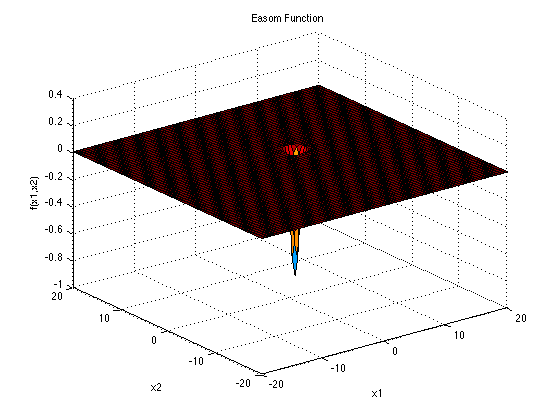
\includegraphics[width=\linewidth]{figures/easom.png}
    \caption{Hàm Easom trong không gian ba chiều}
\end{subfigure}

\vspace{0.8em}

\begin{subfigure}[b]{0.72\linewidth}
    \centering
    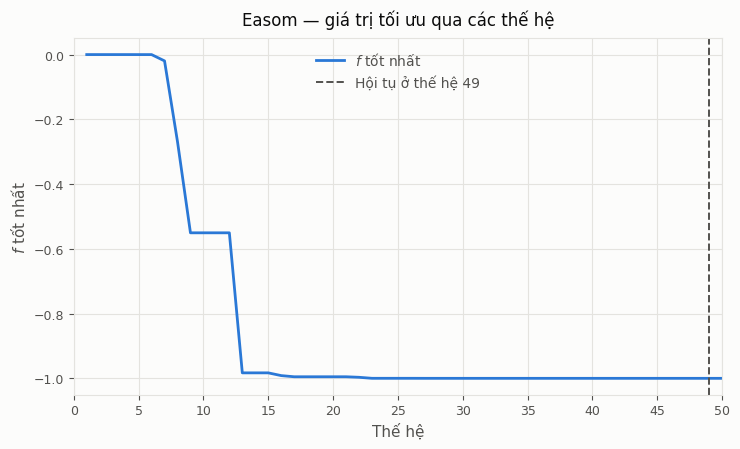
\includegraphics[width=\linewidth]{figures/hoitu_easom.png}
    \caption{Đường hội tụ của GA}
\end{subfigure}
\caption{Hàm Easom: đồ thị trong không gian ba chiều và diễn biến giá trị
tốt nhất qua các thế hệ. Đường nét đứt đánh dấu thế hệ mà GA chốt được
nghiệm tốt nhất.}
\label{fig:easom}
\end{figure}

\textbf{Hàm Rastrigin} có công thức
\begin{equation}
f(x,y) = 20 + x^2 + y^2 - 10\cos(2\pi x) - 10\cos(2\pi y),
\qquad x, y \in [-5.12,\, 5.12],
\label{eq:rastrigin}
\end{equation}
với cực tiểu toàn cục $f(0,0) = 0$. Hai số hạng cosin có chu kỳ bằng
$1$ nên tạo ra một mạng lưới cực tiểu cục bộ nằm xấp xỉ tại các điểm
có tọa độ nguyên; trong miền $[-5.12,\, 5.12]^2$ có khoảng $121$ cực
tiểu cục bộ như vậy, bao quanh dày đặc cực tiểu toàn cục tại gốc tọa
độ. Khó khăn ở đây là bài toán \textit{đa cực trị} điển hình: một
phương pháp cục bộ xuất phát từ điểm ngẫu nhiên gần như chắc chắn rơi
vào giếng gần nhất rồi dừng lại, và giếng đó hầu như không bao giờ là
giếng ở gốc tọa độ. Cái cứu GA ở đây là biên độ đột biến: với
$\sigma = 0{,}08 \times 10{,}24 \approx 0{,}82$, một bước đột biến đủ
lớn để nhảy qua vài ô lưới cực tiểu cục bộ (khoảng cách giữa hai giếng
liền kề là $1$), nên cá thể không bị giam trong một giếng duy nhất.

\begin{figure}[htbp]
\centering
\begin{subfigure}[b]{0.72\linewidth}
    \centering
    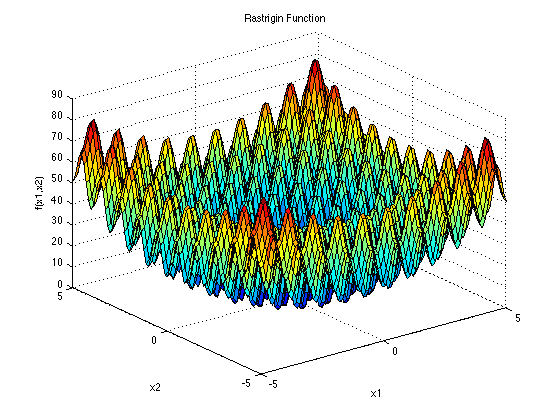
\includegraphics[width=\linewidth]{figures/rastrigin.png}
    \caption{Hàm Rastrigin trong không gian ba chiều}
\end{subfigure}

\vspace{0.8em}

\begin{subfigure}[b]{0.72\linewidth}
    \centering
    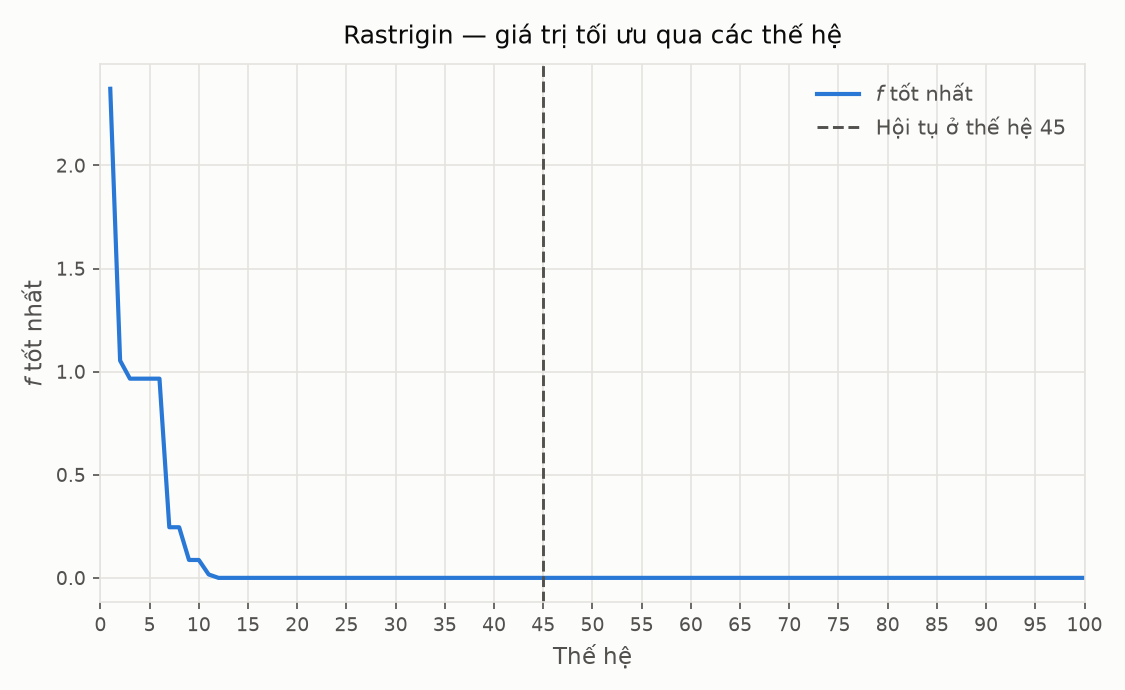
\includegraphics[width=\linewidth]{figures/hoitu_rastrigin.png}
    \caption{Đường hội tụ của GA}
\end{subfigure}
\caption{Hàm Rastrigin: mạng lưới cực tiểu cục bộ dày đặc quanh cực
tiểu toàn cục, và diễn biến giá trị tốt nhất qua các thế hệ.}
\label{fig:rastrigin}
\end{figure}

\textbf{Hàm Rosenbrock} có công thức
\begin{equation}
f(x,y) = (1-x)^2 + 100(y-x^2)^2,
\qquad x \in [-5,\, 10],\ y \in [-5,\, 10],
\label{eq:rosenbrock}
\end{equation}
với cực tiểu toàn cục $f(1,1) = 0$. Khác hẳn bốn hàm còn lại, hàm này
\textit{không} đa cực trị: trên miền hai biến nó chỉ có duy nhất một
cực tiểu, nên không tồn tại bẫy cục bộ nào để thuật toán mắc vào. Khó
khăn nằm ở hình dạng của đáy hàm. Số hạng $100(y-x^2)^2$ phạt rất nặng
mọi sai lệch khỏi đường cong $y = x^2$, tạo thành một thung lũng hẹp
hình quả chuối với vách hai bên dựng đứng, trong khi dọc theo lòng
thung lũng giá trị hàm lại thay đổi rất chậm. Muốn tiến về $(1,1)$,
thuật toán phải thay đổi $x$ và $y$ một cách \textit{phối hợp} sao cho
$y$ luôn bám theo $x^2$; đi lệch nhịp là lập tức đâm vào vách. Cụ thể,
để đạt được $f < 10^{-3}$ thì đồng thời phải có $|1-x| < 0{,}032$ và
$|y-x^2| < 0{,}0032$ --- một dải rất mỏng và cong. Cả hai toán tử của
GA đều không phù hợp với yêu cầu này: lai ghép trộn nội suy theo
\textit{đường thẳng} nối hai cha mẹ, còn đột biến Gauss xê dịch từng
tọa độ một cách \textit{độc lập}, nên không toán tử nào bám được theo
một đường cong. Nói cách khác, với Rosenbrock cái khó không phải là
\textit{tìm ra} vùng chứa nghiệm mà là \textit{dò theo} đáy thung lũng
sau khi đã vào được trong đó.

\begin{figure}[htbp]
\centering
\begin{subfigure}[b]{0.72\linewidth}
    \centering
    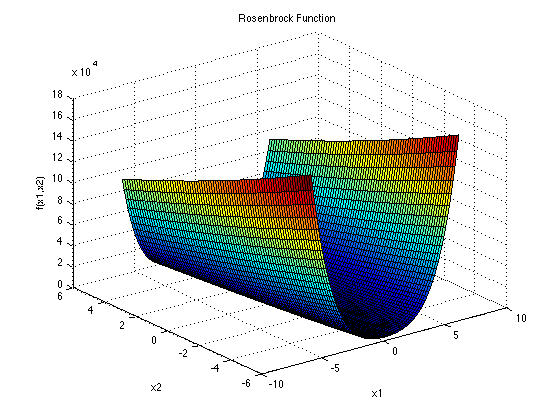
\includegraphics[width=\linewidth]{figures/rosenbrock.png}
    \caption{Hàm Rosenbrock trong không gian ba chiều}
\end{subfigure}

\vspace{0.8em}

\begin{subfigure}[b]{0.72\linewidth}
    \centering
    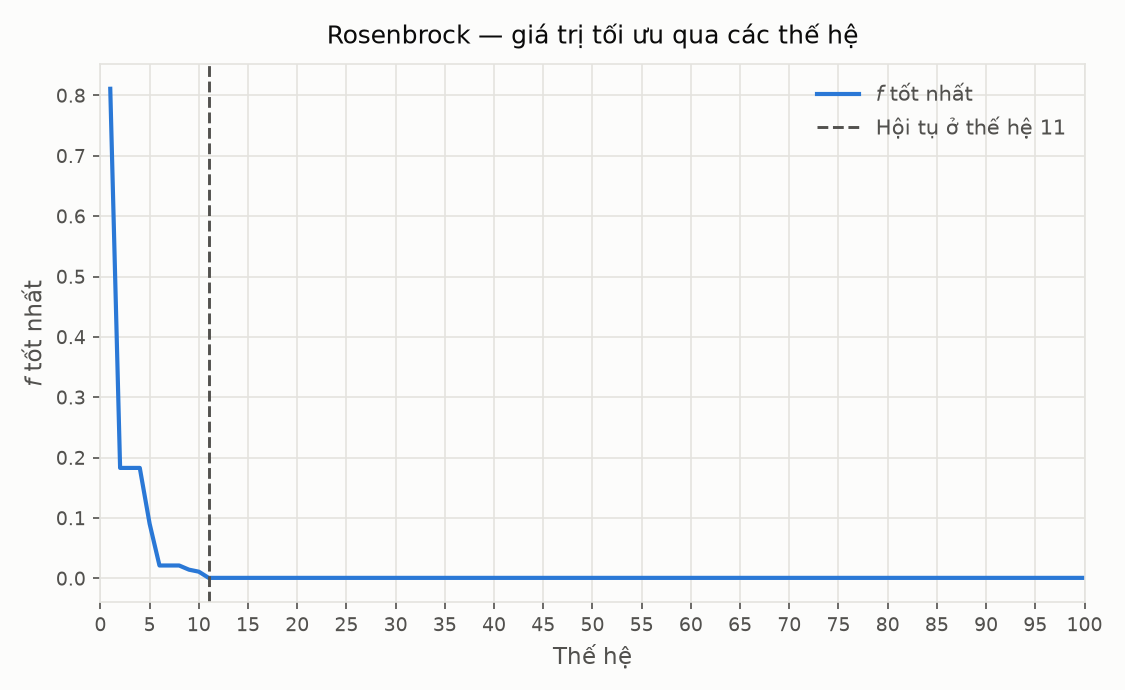
\includegraphics[width=\linewidth]{figures/hoitu_rosenbrock.png}
    \caption{Đường hội tụ của GA}
\end{subfigure}
\caption{Hàm Rosenbrock: thung lũng cong hẹp hình quả chuối, và diễn
biến giá trị tốt nhất qua các thế hệ --- GA chốt kỷ lục ngay ở thế hệ
$11$ rồi không cải thiện thêm trong $89$ thế hệ còn lại.}
\label{fig:rosenbrock}
\end{figure}

\textbf{Hàm Ackley} có công thức
\begin{equation}
\begin{split}
f(x,y) = {} & -20\exp\!\left(-0.2\sqrt{0.5(x^2+y^2)}\right) \\
& - \exp\!\left(0.5\cos(2\pi x) + 0.5\cos(2\pi y)\right) + 20 + e,
\end{split}
\label{eq:ackley}
\end{equation}
với $x, y \in [-32.768,\, 32.768]$ và cực tiểu toàn cục $f(0,0) = 0$.
Hàm này kết hợp hai cấu trúc chồng lên nhau ở hai thang độ khác nhau:
số hạng mũ thứ nhất tạo một cái phễu lớn dốc dần về gốc tọa độ, còn số
hạng cosin phủ lên bề mặt phễu đó vô số gợn sóng cực tiểu cục bộ nhỏ.
Cấu trúc phễu ở thang lớn là thông tin có ích --- nó chỉ đúng hướng
về nghiệm; các gợn sóng ở thang nhỏ mới là bẫy. Do đó Ackley kiểm tra
khả năng \textit{đọc được xu thế toàn cục mà không bị nhiễu cục bộ
đánh lạc hướng}. Với GA, biên độ đột biến
$\sigma = 0{,}08 \times 65{,}536 \approx 5{,}24$ lớn hơn nhiều so với
bước sóng của gợn nhiễu (bằng $1$), nên các gợn sóng gần như trong
suốt đối với quá trình tìm kiếm.

\begin{figure}[htbp]
\centering
\begin{subfigure}[b]{0.72\linewidth}
    \centering
    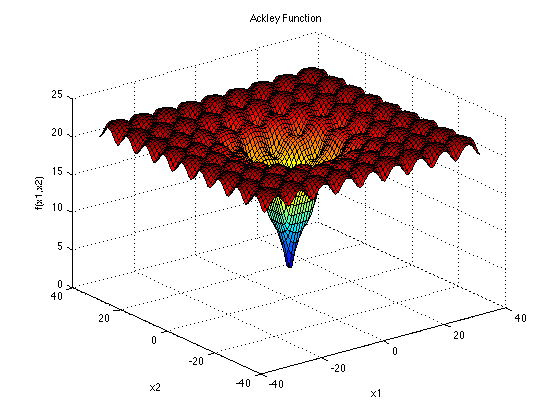
\includegraphics[width=\linewidth]{figures/ackley.png}
    \caption{Hàm Ackley trong không gian ba chiều}
\end{subfigure}

\vspace{0.8em}

\begin{subfigure}[b]{0.72\linewidth}
    \centering
    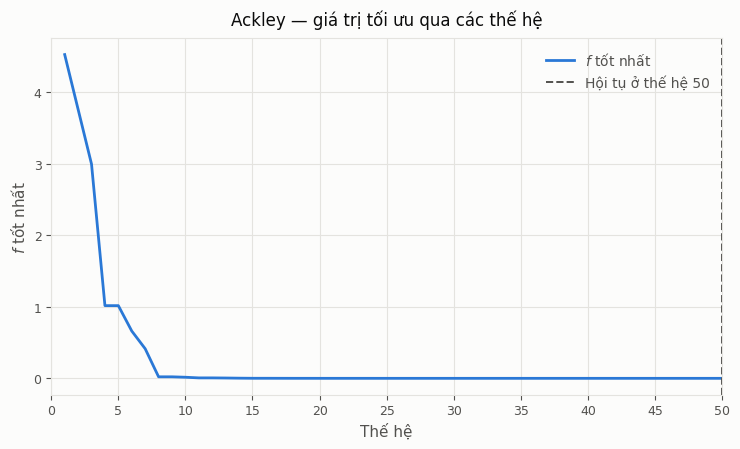
\includegraphics[width=\linewidth]{figures/hoitu_ackley.png}
    \caption{Đường hội tụ của GA}
\end{subfigure}
\caption{Hàm Ackley: phễu lớn ở thang toàn cục phủ gợn sóng cực tiểu
cục bộ ở thang nhỏ, và diễn biến giá trị tốt nhất qua các thế hệ.}
\label{fig:ackley}
\end{figure}

\textbf{Hàm Schwefel} có công thức
\begin{equation}
f(x,y) = 837.9658 - x\sin\sqrt{|x|} - y\sin\sqrt{|y|},
\qquad x, y \in [-500,\, 500],
\label{eq:schwefel}
\end{equation}
với cực tiểu toàn cục $f(420.9687,\, 420.9687) \approx 0$. Đây là hàm
được thiết kế để \textit{đánh lừa}: các cực tiểu cục bộ của nó phân bố
không đều, và điều nguy hiểm là cực tiểu cục bộ tốt thứ nhì lại nằm
rất xa cực tiểu toàn cục trong không gian tìm kiếm. Hệ quả là thông
tin cục bộ dẫn đường sai --- một thuật toán càng khai thác sớm và
càng mạnh vùng đang có vẻ tốt thì càng bị kéo ra xa nghiệm đúng. Thêm
vào đó, cực tiểu toàn cục nằm ở $420{,}97$, tức sát biên $500$ của
miền tìm kiếm, nên những cài đặt cắt hoặc co cá thể về phía tâm miền
sẽ bỏ sót nó. Hàm này vì vậy kiểm tra khả năng duy trì thăm dò trên
diện rộng và không cam kết quá sớm vào một vùng.

\begin{figure}[htbp]
\centering
\begin{subfigure}[b]{0.72\linewidth}
    \centering
    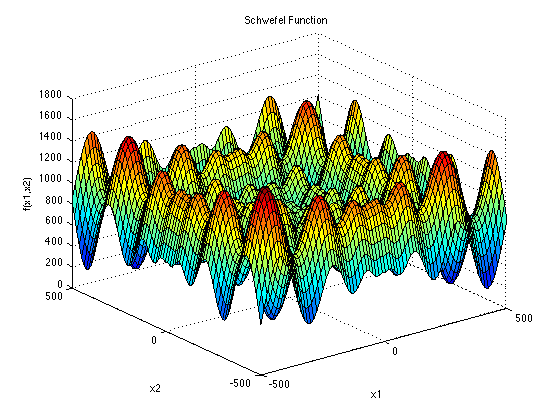
\includegraphics[width=\linewidth]{figures/schwefel.png}
    \caption{Hàm Schwefel trong không gian ba chiều}
\end{subfigure}

\vspace{0.8em}

\begin{subfigure}[b]{0.72\linewidth}
    \centering
    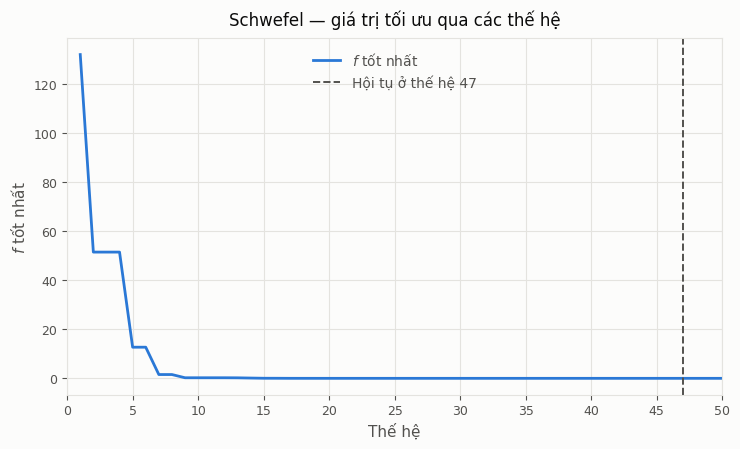
\includegraphics[width=\linewidth]{figures/hoitu_schwefel.png}
    \caption{Đường hội tụ của GA}
\end{subfigure}
\caption{Hàm Schwefel: cực tiểu toàn cục nằm gần biên miền tìm kiếm,
xa vùng trông có vẻ tốt quanh gốc tọa độ, và diễn biến giá trị tốt
nhất qua các thế hệ.}
\label{fig:schwefel}
\end{figure}

Với mỗi hàm, GA mã hóa số thực (lai ghép trộn BLX-$\alpha$ với
$\alpha \in [-0{,}25;\, 1{,}25]$, đột biến Gauss với xác suất $0{,}15$
trên mỗi gene và $\sigma$ bằng $0{,}08$ lần bề rộng miền, chọn lọc
giải đấu theo thứ hạng với $k = 3$, giữ lại $2$ cá thể tinh hoa mỗi
thế hệ --- theo Mục~\ref{sec:toan-tu-cot-loi}) được chạy một lần với
quần thể $500$ cá thể trong $100$ thế hệ, hạt giống ngẫu nhiên cố định
bằng $42$ để kết quả tái lập được. Cá thể được cắt về miền tìm kiếm
sau mỗi phép lai ghép và đột biến, vì ở đây miền đóng vai trò miền xác
định của bài toán. Thuật toán không có tiêu chí dừng sớm: vòng lặp
luôn chạy đủ $100$ thế hệ. Cột \textit{số thế hệ thỏa mãn} trong
Bảng~\ref{tab:kq-khong-rang-buoc} vì vậy không phải thế hệ mà thuật
toán dừng lại, mà là thế hệ sớm nhất đạt được giá trị $f^{*}$ cuối
cùng --- tức lần cuối cùng kỷ lục được cải thiện.

\begin{table}[htbp]
\centering
\caption{Kết quả GA trên năm hàm benchmark không ràng buộc}
\label{tab:kq-khong-rang-buoc}
\small
\setlength{\tabcolsep}{5pt}
\begin{tabular}{lccccc}
\toprule
\textbf{Hàm} & \textbf{Thời gian} & \textbf{Số thế hệ}
& \textbf{$f^{*}$} & \textbf{$x^{*}$} & \textbf{$y^{*}$} \\
& \textbf{(s)} & \textbf{thỏa mãn} & & & \\
\midrule
Easom      & $1.3619$ & $51$ & $-1.0000000000$      & $3.141593$              & $3.141593$               \\
Rastrigin  & $1.3876$ & $45$ & $0.0000000000$       & $8.00\times10^{-10}$    & $-2.11\times10^{-9}$     \\
Rosenbrock & $1.4194$ & $11$ & $0.0009051359$       & $1.008839$              & $1.014881$               \\
Ackley     & $1.5411$ & $76$ & $0.0000000000$       & $-9.22\times10^{-17}$   & $-2.99\times10^{-16}$    \\
Schwefel   & $1.4160$ & $52$ & $2.5455\times10^{-5}$ & $420.968746$           & $420.968746$             \\
\bottomrule
\end{tabular}
\end{table}

GA tìm đúng, hoặc gần đúng đến sai số không đáng kể, cực tiểu toàn cục
trên cả năm hàm --- kể cả Easom và Schwefel, hai hàm được thiết kế
riêng để đánh lừa các thuật toán chỉ khai thác thông tin cục bộ quanh
điểm hiện tại. Kết quả này minh chứng trực tiếp cho ưu điểm cốt lõi
của tìm kiếm dựa trên quần thể đã trình bày ở
Mục~\ref{subsec:ho-thuat-toan-tien-hoa}: vì GA duy trì $500$ cá thể
trải rộng trên không gian tìm kiếm thay vì một điểm duy nhất, nó không
phụ thuộc vào việc điểm khởi tạo có nằm gần cực tiểu toàn cục hay
không, khác với các phương pháp gradient cổ điển. Với Rastrigin và
Ackley, GA về đúng $0$ trong giới hạn biểu diễn số thực dấu phẩy động.

Rosenbrock là ngoại lệ duy nhất, và cách nó khác biệt lại soi sáng
đúng điểm mạnh cũng như điểm yếu của GA. Sai số $9{,}05\times10^{-4}$
của nó lớn hơn bốn hàm còn lại nhiều bậc độ lớn, mặc dù đây là hàm
\textit{duy nhất} trong năm hàm không hề có bẫy cực tiểu cục bộ.
Đường hội tụ ở Hình~\ref{fig:rosenbrock} cho thấy rõ cơ chế: giá trị
tốt nhất tụt rất nhanh trong mười thế hệ đầu rồi chốt lại ở thế hệ
$11$ và đứng yên suốt $89$ thế hệ còn lại. Nghĩa là GA lọt vào đúng
thung lũng gần như tức thì, nhưng sau đó không nhích thêm được nữa.
Đối chiếu với Ackley --- hàm mà GA cải thiện kỷ lục rải rác cho tới
tận thế hệ $76$ --- có thể thấy hai kiểu khó khăn hoàn toàn khác nhau:
Rastrigin, Ackley, Easom và Schwefel khó ở chỗ \textit{tìm ra} đúng
vùng chứa nghiệm, còn Rosenbrock khó ở chỗ \textit{dò theo} một cấu
trúc cong sau khi đã tìm ra vùng đó.

Sự phân đôi này phản ánh bản chất của các toán tử tiến hóa ngẫu nhiên
đẳng hướng: chúng rất mạnh trong việc định vị một vùng rộng trên không
gian tìm kiếm, nhưng yếu trong việc tinh chỉnh dọc theo một hướng ưu
tiên hẹp. Đây chính là lý do các thuật toán lai ghép GA với tìm kiếm
cục bộ (memetic algorithm) tồn tại --- và cũng là cách tiếp cận được
áp dụng cho bài toán người du lịch ở Mục~\ref{sec:ud-tsp}, nơi GA
thuần túy được bổ sung thêm bước tối ưu cục bộ 2-opt để xử lý đúng
phần việc mà lai ghép và đột biến ngẫu nhiên làm không tốt.

\section{Tối ưu có ràng buộc: So sánh GA với SciPy SLSQP}
\label{sec:ud-co-rang-buoc}

Năm bài toán tối ưu có ràng buộc được lựa chọn để bao quát các dạng
ràng buộc và tính chất hàm mục tiêu khác nhau, từ tuyến tính tuyệt đối
đến phi tuyến.

\textbf{Bài toán 1 — Entropy tối đa.} Đây là bài toán ``con xúc xắc bị
làm lệch'' của Jaynes: tìm phân phối xác suất $x_1,\ldots,x_6$ của một
con xúc xắc sáu mặt có entropy lớn nhất, biết trước kỳ vọng
$E[X]=4.5$. Sau khi đổi dấu để đưa về bài toán cực tiểu hóa (vì
$\max H(x) \equiv \min -H(x)$), phát biểu toán học là
\begin{equation}
\min_{x \in \mathbb{R}^6} f(x) = \sum_{i=1}^{6} x_i \ln x_i
\quad \text{s.t.} \quad
\sum_{i=1}^{6} x_i = 1,\quad
\sum_{i=1}^{6} i\, x_i = 4.5,\quad
x_i \ge 0.
\label{eq:entropy}
\end{equation}
Hai ràng buộc đẳng thức phải được thỏa mãn đồng thời, khiến miền khả
thi chỉ còn là giao tuyến của hai siêu phẳng trong $\mathbb{R}^6$.

\textbf{Bài toán 2 — Điểm gần nhất trong miền ràng buộc.} Cho một điểm
$(5,\, 4,\, -2)$ nằm ngoài miền ràng buộc, tìm điểm $(x,y,z)$ trong
miền ràng buộc gần điểm đó nhất theo khoảng cách Euclid bình phương —
tức là bài toán chiếu một điểm lên một tập lồi:
\begin{equation}
\min_{x,y,z} f(x,y,z) = (x-5)^2+(y-4)^2+(z+2)^2
\quad \text{s.t.} \quad
x+2y+z=4,\quad
x^2+y^2\le9,\quad
z\ge0.
\label{eq:nearest-point}
\end{equation}
Miền ràng buộc là giao của một mặt phẳng, một hình trụ, và một nửa
không gian.

\textbf{Bài toán 3 — Quy hoạch tuyến tính.} Hàm mục tiêu và mọi ràng
buộc đều tuyến tính:
\begin{equation}
\max_{x,y,z} f(x,y,z) = 3x+5y-2z
\quad \text{s.t.} \quad
x+2y+z=10,\quad
2x+y\le8,\quad
x,y,z\ge0.
\label{eq:lp}
\end{equation}
Vì là quy hoạch tuyến tính (LP) thuần túy, nghiệm tối ưu chắc chắn nằm
tại một đỉnh của miền đa diện lồi xác định bởi các ràng buộc.

\textbf{Bài toán 4 — Quy hoạch bình phương.} Hàm mục tiêu bậc hai lồi,
ràng buộc tuyến tính:
\begin{equation}
\min_{x,y,z} f(x,y,z) = x^2+2y^2+z^2-4x-6y
\quad \text{s.t.} \quad
x+y+2z=5,\quad
x+y\le3,\quad
x,y,z\ge0.
\label{eq:qp}
\end{equation}
Vì hàm mục tiêu lồi và miền ràng buộc lồi, bài toán này (quy hoạch
bình phương — QP) có đúng một cực tiểu toàn cục.

\textbf{Bài toán 5 — Tối ưu lồi phi tuyến.} Hàm mục tiêu là tổng hai
hàm mũ, khác hẳn tính chất tuyến tính từng khúc của bốn bài toán trên:
\begin{equation}
\min_{x,y} f(x,y) = e^{-x}+e^{-2y}
\quad \text{s.t.} \quad
2x+3y=6,\quad
x^2+y^2\le4,\quad
x,y\ge0.
\label{eq:convex-exp}
\end{equation}
Cả hàm mục tiêu lẫn miền ràng buộc đều lồi nên bài toán vẫn có đúng
một cực tiểu toàn cục, dù không còn là dạng tuyến tính hay bình phương.

GA cho cả năm bài toán này sử dụng chiến lược xử lý ràng buộc đã giới
thiệu ở Mục~\ref{subsec:ham-thich-nghi} — kết hợp quy tắc khả thi Deb
với ngưỡng $\varepsilon$ giảm dần theo thời gian, thay vì hàm phạt
tĩnh — chạy với quần thể $1000$ cá thể trong tối đa $500$ thế hệ, lặp
lại ba lần độc lập. Đối trọng so sánh là SciPy SLSQP, một phương pháp
tối ưu dựa trên gradient giải theo điều kiện KKT, được chạy từ $30$
điểm khởi tạo ngẫu nhiên khác nhau để giảm rủi ro hội tụ về một cực
tiểu cục bộ thay vì cực tiểu toàn cục. Kết quả tốt nhất của mỗi phương
pháp được trình bày ở Bảng~\ref{tab:kq-co-rang-buoc}.

\begin{table}[htbp]
\centering
\caption{Kết quả GA và SciPy SLSQP trên năm bài toán tối ưu có ràng buộc}
\label{tab:kq-co-rang-buoc}
\begin{tabular}{lcc}
\toprule
\textbf{Bài toán} & \textbf{GA ($f^{*}$)} & \textbf{SLSQP ($f^{*}$)} \\
\midrule
1. Entropy tối đa            & $-1.5985825694$  & $-1.6135810982$ \\
2. Điểm gần nhất             & $20.3497958340$  & $20.2756044350$ \\
3. Quy hoạch tuyến tính (LP) & $-25.9149581523$ & $-26.0000000000$ \\
4. Quy hoạch bình phương (QP)& $-7.3329937494$  & $-7.3333333333$ \\
5. Tối ưu lồi phi tuyến      & $0.3565975317$   & $0.3565154830$  \\
\bottomrule
\end{tabular}
\end{table}

SLSQP đạt kết quả nhỉnh hơn GA một chút ở cả năm bài toán. Điều này
đúng như kỳ vọng lý thuyết, vì cả năm bài toán đều lồi và có hàm mục
tiêu khả vi — chính là điều kiện lý tưởng nhất cho một phương pháp dựa
trên gradient và điều kiện KKT như SLSQP, trong khi GA không khai thác
được thông tin đạo hàm này để tinh chỉnh nghiệm ở bước cuối. Tuy vậy,
khoảng cách giữa hai phương pháp rất nhỏ: GA đạt trong khoảng
$0.01\%$ đến $1\%$ so với SLSQP ở bốn trong năm bài toán; riêng bài
toán 3 (LP) có sai số tương đối lớn hơn một chút, vì nghiệm tối ưu của
LP luôn nằm đúng tại một đỉnh sắc cạnh của miền đa diện — một điểm mà
các toán tử lai ghép/đột biến liên tục của GA khó tiệm cận chính xác
tuyệt đối hơn so với việc dò theo một đường cong trơn. Nhìn chung, kết
quả cho thấy GA vẫn xấp xỉ tốt cả năm bài toán dù không dùng đến đạo
hàm. Điều này có ý nghĩa thực tiễn quan trọng: trong các bài toán mà
hàm mục tiêu không khả vi hoặc không lồi — nơi SLSQP không còn đảm bảo
hội tụ đúng — khả năng xấp xỉ tốt của GA mà không cần thông tin đạo
hàm trở thành một lợi thế thực sự, như sẽ thấy rõ hơn ở hai bài toán
tiếp theo.

\section{Bài toán Người du lịch: GA hoán vị kết hợp Tìm kiếm Cục bộ}
\label{sec:ud-tsp}

Bài toán người du lịch (Traveling Salesman Problem — TSP) được phát
biểu như sau: cho $n$ địa điểm và ma trận khoảng cách
$D = (d_{ij})_{n\times n}$ giữa mọi cặp địa điểm, tìm một hoán vị
$\pi = (\pi_1, \ldots, \pi_n)$ của $n$ địa điểm sao cho tổng độ dài lộ
trình khép kín đi qua tất cả các địa điểm đúng một lần là nhỏ nhất:
\begin{equation}
\min_{\pi} L(\pi) = \sum_{k=1}^{n-1} d_{\pi_k, \pi_{k+1}} + d_{\pi_n, \pi_1}.
\label{eq:tsp}
\end{equation}
Bài toán này được mã hóa dưới dạng hoán vị đã giới thiệu ở
Mục~\ref{subsec:ma-hoa}: mỗi cá thể của GA chính là một hoán vị $\pi$,
dùng lai ghép Order Crossover (OX) và đột biến Swap (Mục~\ref{sec:toan-tu-cot-loi})
thay cho các toán tử số thực ở hai mục trước.

Để đánh giá khách quan trên dữ liệu thực thay vì các ví dụ tự tạo quy
mô nhỏ, ba bộ dữ liệu chuẩn từ thư viện benchmark TSPLIB95 [9] được sử
dụng: berlin52 ($n=52$ địa điểm tại Berlin), rd100 ($n=100$ địa điểm
ngẫu nhiên), và ch150 ($n=150$ địa điểm). Mỗi bộ dữ liệu đều có kèm
theo lộ trình tối ưu đã được công bố, dùng làm mốc đối chiếu khách
quan thay cho phương pháp vét cạn — vốn cần thử $(n-1)!$ hoán vị và
trở nên bất khả thi về mặt tính toán ngay từ $n$ vài chục.

Thử nghiệm ban đầu với GA hoán vị thuần túy (chỉ dùng OX và Swap) cho
kết quả chênh lệch rất lớn so với nghiệm tối ưu đã công bố, từ $20\%$
đến $84\%$ tùy bộ dữ liệu và tăng dần theo số địa điểm $n$. Nguyên
nhân là hai toán tử OX và Swap không có cơ chế sửa các đoạn đường bị
cắt chéo nhau trong lộ trình — một lộ trình càng có nhiều địa điểm thì
càng dễ chứa những đoạn cắt chéo như vậy, và OX/Swap chỉ có thể tạo ra
một cấu hình mới ngẫu nhiên chứ không chủ động ``gỡ'' đoạn cắt chéo đó.
Để khắc phục hạn chế này, một chiến lược lai giữa GA và tìm kiếm cục bộ
(\textit{memetic algorithm}) được áp dụng: sau mỗi thế hệ, một tỉ lệ cá
thể tốt nhất trong quần thể được tinh chỉnh thêm bằng phép tìm kiếm cục
bộ \textbf{2-opt} — xét lần lượt từng cặp cạnh trong lộ trình, hoán đổi
hai cạnh đó nếu việc hoán đổi làm giảm tổng độ dài — trước khi tiếp tục
vòng lặp tiến hóa (chọn lọc, lai ghép, đột biến) như bình thường. Với
tỉ lệ tinh chỉnh bằng khoảng $5\%$ quần thể mỗi thế hệ, cả ba bộ dữ
liệu đều đạt đúng lộ trình tối ưu đã công bố, như trình bày ở
Bảng~\ref{tab:kq-tsp}.

\begin{table}[htbp]
\centering
\caption{Kết quả GA kết hợp 2-opt trên ba bộ dữ liệu TSPLIB95}
\label{tab:kq-tsp}
\begin{tabular}{lcccc}
\toprule
\textbf{Bộ dữ liệu} & \textbf{Số địa điểm ($n$)} & \textbf{Nghiệm tối ưu} & \textbf{GA} & \textbf{Đạt được ở thế hệ} \\
\midrule
berlin52 & 52  & 7542 & 7542 & 8/50  \\
rd100    & 100 & 7910 & 7910 & 48/50 \\
ch150    & 150 & 6528 & 6528 & 37/50 \\
\bottomrule
\end{tabular}
\end{table}

Trong quá trình hiệu chỉnh tham số, một quan sát quan trọng được ghi
nhận: tỉ lệ cá thể được tinh chỉnh bằng 2-opt cần được đặt theo
\textit{phần trăm} của quần thể chứ không phải theo một số lượng cố
định. Cụ thể, khi giữ nguyên số lượng cá thể được tinh chỉnh ở một
con số tuyệt đối nhưng tăng kích thước quần thể lên, kết quả trở nên
tệ hơn so với quần thể nhỏ — nguyên nhân là vì trong một quần thể lớn,
số cá thể đã qua tinh chỉnh chiếm tỉ lệ quá nhỏ nên khó lan gen tốt ra
phần còn lại của quần thể thông qua phép chọn lọc. Quan sát này cho
thấy các tham số của một chiến lược lai giữa GA và tìm kiếm cục bộ
không thể được chọn độc lập với nhau, mà phải cân chỉnh tương thích
với quy mô quần thể.

\section{Hồi quy Ký hiệu bằng Lập trình Di truyền}
\label{sec:ud-symbolic-regression}

Ứng dụng cuối cùng minh họa Lập trình Di truyền (Mục~\ref{sec:gp}) cho
bài toán hồi quy ký hiệu trên dữ liệu vật lý thực: các phép đo mật độ
hạt, vận tốc, và từ trường của gió mặt trời do vệ tinh WIND của NASA
ghi nhận. Ba thành phần từ trường đo được là $B_X, B_Y, B_Z$, và mật độ
hạt đo được là $n$. Từ bốn đại lượng này, hai đại lượng vật lý phái
sinh được chọn làm mục tiêu dự đoán cho GP:
\begin{equation}
|B|^2 = B_X^2+B_Y^2+B_Z^2
\qquad \text{(bình phương độ lớn từ trường)},
\label{eq:b-squared}
\end{equation}
\begin{equation}
V_A^2 \propto \frac{|B|^2}{n}
\qquad \text{(vận tốc Alfvén bình phương)}.
\label{eq:alfven-squared}
\end{equation}
Đại lượng thứ nhất là một quan hệ tổng bình phương (dạng Pythagore)
giữa ba biến đo được; đại lượng thứ hai kết hợp thêm một phép chia cho
biến mật độ hạt.

Điểm mấu chốt khiến hai đại lượng này trở thành phép thử công bằng cho
GP là: quan hệ tổng bình phương ở Phương trình~\eqref{eq:b-squared}
\textit{không thể} tuyến tính hóa bằng phép biến đổi logarit như các
quan hệ dạng lũy thừa thông thường, vì $B_X, B_Y, B_Z$ có thể mang giá
trị âm nên không lấy logarit được. Do đó, Hồi quy Tuyến tính áp dụng
trực tiếp trên ba đặc trưng thô $B_X, B_Y, B_Z$ gần như chắc chắn
không thể biểu diễn được cấu trúc bậc hai này, vì mô hình tuyến tính
chỉ có thể biểu diễn một tổ hợp tuyến tính của chính các đặc trưng đó,
không tự sinh ra được số hạng bậc hai. Ngược lại, GP có thể tự xây
dựng số hạng bậc hai bằng cách nhân một biến với chính nó ngay trong
cây biểu thức, mà không cần được cung cấp trước các đặc trưng
$B_X^2, B_Y^2, B_Z^2$ như một phép biến đổi thủ công. Kết quả đối
chiếu hai phương pháp trên tập kiểm tra được trình bày ở
Bảng~\ref{tab:kq-symbolic-regression}.

\begin{table}[htbp]
\centering
\caption{Kết quả Hồi quy Tuyến tính và GP trên hai đại lượng vật lý phái sinh}
\label{tab:kq-symbolic-regression}
\begin{tabular}{llccc}
\toprule
\textbf{Đại lượng} & \textbf{Phương pháp} & \textbf{MAE} & \textbf{RMSE} & \textbf{$R^2$} \\
\midrule
\multirow{2}{*}{$|B|^2$}
    & Hồi quy Tuyến tính & 15.1284 & 19.9825 & 0.4784 \\
    & GP (hồi quy ký hiệu) & 4.1820 & 6.0779 & 0.9517 \\
\addlinespace
\multirow{2}{*}{$V_A^2$}
    & Hồi quy Tuyến tính & 2.7376 & 3.6804 & 0.4629 \\
    & GP (hồi quy ký hiệu) & 1.0554 & 1.5486 & 0.9049 \\
\bottomrule
\end{tabular}
\end{table}

Kết quả cho thấy chênh lệch rõ rệt và nhất quán trên cả hai đại lượng.
Hồi quy Tuyến tính chỉ giải thích được khoảng $46\%$ đến $48\%$ phương
sai của dữ liệu ($R^2 \approx 0.46$–$0.48$), trong khi GP đạt trên
$90\%$ ($R^2 \approx 0.90$–$0.95$); đồng thời sai số dự đoán (MAE,
RMSE) của GP chỉ còn chưa đến một phần ba so với Hồi quy Tuyến tính ở
cả hai đại lượng. Đây là kết quả trái ngược hẳn với các bài toán hồi
quy dạng lũy thừa từng được thử nghiệm trong quá trình thực hiện tiểu
luận — ví dụ định luật Kepler III hay áp suất động của gió mặt trời —
là những quan hệ trở thành tuyến tính tuyệt đối sau khi biến đổi
logarit, khiến Hồi quy Tuyến tính ở các bài toán đó luôn đạt hoặc vượt
GP. Sự tương phản giữa hai nhóm kết quả khẳng định đúng giả thuyết ban
đầu: lợi thế thực sự của GP so với hồi quy cổ điển chỉ bộc lộ rõ khi
quan hệ cần khám phá có cấu trúc phi tuyến mà phép biến đổi đặc trưng
thủ công thông thường, như logarit, không xử lý được.

\section{Tổng kết Chương}
\label{sec:ud-tong-ket}

Bốn thực nghiệm trên minh họa một đặc điểm xuyên suốt của Thuật toán
Di truyền: tính linh hoạt cao nhờ khả năng thích ứng với nhiều cách mã
hóa khác nhau — số thực ở Mục~\ref{sec:ud-khong-rang-buoc}
và~\ref{sec:ud-co-rang-buoc}, hoán vị ở Mục~\ref{sec:ud-tsp}, và cây
biểu thức ở Mục~\ref{sec:ud-symbolic-regression}. Đổi lại tính linh
hoạt đó là hiệu quả thấp hơn các phương pháp chuyên dụng khi bài toán
có sẵn một cấu trúc mà phương pháp đó khai thác được: SLSQP khai thác
tính khả vi và tính lồi của năm bài toán ở
Mục~\ref{sec:ud-co-rang-buoc}. Ngược lại, ở những bài toán mà cấu trúc
đó không có sẵn, hoặc phương pháp cổ điển tương ứng không còn đủ mạnh
— bài toán người du lịch quy mô lớn cần bổ sung tìm kiếm cục bộ mới
đạt được nghiệm tối ưu, hay quan hệ phi tuyến dạng tổng bình phương mà
Hồi quy Tuyến tính không thể biểu diễn được — GA và GP thể hiện rõ giá
trị thực tiễn của một phương pháp tìm kiếm không đặt giả định trước về
cấu trúc bài toán.


% ================= KẾT LUẬN =================
% ============================================================
% KẾT LUẬN (không đánh số chương, ngang hàng với Tài liệu tham khảo)
% ============================================================
\chapter*{Kết luận}
\addcontentsline{toc}{chapter}{Kết luận}
\label{chap:ket-luan}

\noindent\textbf{Tóm tắt}
\medskip

Tiểu luận đã trình bày cơ sở lý thuyết của Thuật toán Di truyền
và mở rộng của nó là Lập trình Di truyền, sau đó minh họa cả hai
phương pháp qua bốn thực nghiệm cụ thể. Chương~\ref{chap:co-so-ly-thuyet}
xây dựng khung lý thuyết theo trình tự: tổng quan bài toán tối ưu và
họ thuật toán tiến hóa; cơ sở khoa học của GA với ba cách mã hóa cá
thể (nhị phân, số thực, hoán vị); các thành phần cốt lõi của một vòng
lặp tiến hóa (hàm thích nghi, chọn lọc, lai ghép, đột biến, elitism);
quy trình thuật toán và điều kiện dừng; và cuối cùng là GP với mã hóa
dạng cây biểu thức.

Trên nền tảng đó, Chương~\ref{chap:ung-dung} áp dụng GA cho ba nhóm
bài toán tối ưu số — không ràng buộc trên năm hàm benchmark kinh điển,
có ràng buộc trên năm bài toán chuẩn CEC 2006, và bài toán người du
lịch kết hợp 2-opt local search theo mô hình memetic algorithm — đối
chiếu trực tiếp với các mốc nghiệm tối ưu đã công bố. Ở cả ba nhóm,
GA (khi cần thiết được hỗ trợ thêm bởi tìm kiếm cục bộ) đều đạt hoặc
tiệm cận nghiệm tối ưu đã biết. Riêng ứng dụng thứ tư dùng GP cho bài
toán hồi quy symbolic, dự đoán nhiệt độ điểm sương từ nhiệt độ không
khí và độ ẩm tương đối trên dữ liệu thời tiết thực tế, đạt
$R^2 = 0.9967$ trên tập kiểm tra và tìm ra một biểu thức tường minh
phản ánh đúng cấu trúc phi tuyến (logarit, phép chia lồng nhau) của
quan hệ vật lý thật (công thức Magnus), thay vì chỉ đưa ra một mô hình
dự đoán dạng hộp đen.

\bigskip
\noindent\textbf{Hạn chế}
\medskip

Bên cạnh những kết quả đạt được, tiểu luận vẫn còn một số hạn chế cần
được xem xét. Thứ nhất, tính linh hoạt của GA/GP đi kèm với việc không
khai thác trước các đặc trưng cấu trúc của bài toán, do đó hiệu quả tìm
kiếm có thể chưa cao trong một số trường hợp. Đối với các bài toán tối
ưu có ràng buộc, GA thuần túy có thể gặp khó khăn trong việc tìm kiếm
các nghiệm nằm sát biên của miền khả thi. Kết quả thực nghiệm trên các
bài toán CEC 2006 cho thấy việc bổ sung cơ chế tìm kiếm cục bộ có thể
giúp thuật toán tiếp cận nghiệm tốt hơn. Tương tự, đối với bài toán
người du lịch (TSP) có quy mô lớn, việc kết hợp GA với các phép cải
thiện nghiệm như 2-opt giúp quá trình hội tụ nhanh hơn và đưa nghiệm
thu được đến gần nghiệm tối ưu.

Thứ hai, trong bài toán hồi quy biểu thức bằng GP, không gian biểu diễn
hằng số của các nút lá còn bị giới hạn. Cụ thể, engine GP được xây dựng
trong tiểu luận chỉ cho phép các hằng số nằm trong khoảng $[-2,2]$.
Điều này gây khó khăn khi biểu diễn chính xác các hằng số có độ lớn
lớn hơn, chẳng hạn các hằng số $a, b$ xuất hiện trong công thức Magnus.
Để biểu diễn những giá trị này, GP phải kết hợp nhiều nút và phép toán
trung gian, từ đó làm tăng kích thước cây và tiêu tốn ngân sách độ sâu
vốn cần thiết cho việc xây dựng cấu trúc chính của biểu thức. Đây cũng
là một trong những nguyên nhân khiến GP chưa thể khôi phục chính xác
tuyệt đối công thức Magnus.

Thứ ba, phạm vi thực nghiệm của tiểu luận còn tương đối hạn chế. Các
thí nghiệm hiện mới được thực hiện với một thiết lập ngẫu nhiên cố
định cho mỗi cấu hình tham số, do đó chưa đánh giá đầy đủ mức độ ổn
định của thuật toán trước sự thay đổi của quá trình khởi tạo. Bên cạnh
đó, quy mô của các bài toán được khảo sát, chẳng hạn số chiều trong các
bài toán tối ưu có ràng buộc, số địa điểm trong TSP hay số lượng và
đặc trưng của biến đầu vào trong hồi quy biểu thức, vẫn còn tương đối
nhỏ so với nhiều bài toán thực tế phức tạp. Vì vậy, khả năng mở rộng và
tính ổn định của GA/GP trên các bài toán có quy mô lớn hơn vẫn cần
được đánh giá thêm.

\bigskip
\noindent\textbf{Hướng phát triển}
\medskip

Từ những hạn chế đã nêu, tiểu luận đề xuất một số hướng phát triển cho
các nghiên cứu tiếp theo:

\begin{itemize}
    \item Đối với hạn chế về hiệu quả tìm kiếm, có thể nghiên cứu việc
    kết hợp GA với các phương pháp tìm kiếm cục bộ phù hợp với từng
    bài toán. Bên cạnh 2-opt cho TSP, có thể áp dụng các phương pháp
    tối ưu dựa trên gradient đối với những bài toán có hàm mục tiêu và
    ràng buộc khả vi. Đồng thời, có thể sử dụng cơ chế tham số thích
    ứng để tự điều chỉnh tỷ lệ lai ghép, tỷ lệ đột biến và kích thước
    quần thể theo tiến trình hội tụ.

    \item Đối với hạn chế về khả năng biểu diễn hằng số trong GP, có
    thể bổ sung bước tối ưu riêng cho các hằng số tại nút lá sau khi
    cấu trúc cây được xác định. Các phương pháp như least-squares hoặc
    gradient descent có thể được sử dụng để tinh chỉnh các hằng số,
    thay vì chỉ dựa vào đột biến ngẫu nhiên trong một khoảng giá trị
    cố định.

    \item Đối với hạn chế về phạm vi thực nghiệm, nên thực hiện mỗi
    cấu hình nhiều lần với các quá trình khởi tạo ngẫu nhiên khác
    nhau và báo cáo giá trị trung bình cùng độ lệch chuẩn. Đồng thời,
    có thể tăng quy mô bài toán, chẳng hạn số chiều, số địa điểm trong
    TSP và số lượng đặc trưng đầu vào, nhằm đánh giá tốt hơn tính ổn
    định và khả năng mở rộng của GA/GP.
\end{itemize}


% ================= TÀI LIỆU THAM KHẢO =================
% ============================================================
% TÀI LIỆU THAM KHẢO
%
% Hiện chỉ liệt kê các tài liệu được trích dẫn trong Chương 1. Danh sách
% sẽ được bổ sung khi Chương 2 (thực nghiệm) được viết.
% ============================================================
\chapter*{Tài liệu tham khảo}
\addcontentsline{toc}{chapter}{Tài liệu tham khảo}

\begin{enumerate}

\item Holland, J. H. (1975). \textit{Adaptation in Natural and Artificial Systems}. University of Michigan Press, Ann Arbor. (2nd Edition, MIT Press, 1992.)

\item Goldberg, D. E. (1989). \textit{Genetic Algorithms in Search, Optimization, and Machine Learning}. Addison-Wesley.

\item Deb, K. (2000). An efficient constraint handling method for genetic algorithms. \textit{Computer Methods in Applied Mechanics and Engineering}, 186(2--4), 311--338.

\item Takahama, T., \& Sakai, S. (2010, July). Constrained optimization by the $\varepsilon$ constrained differential evolution with an archive and gradient-based mutation. In \textit{IEEE Congress on Evolutionary Computation} (pp. 1--9). IEEE.

\item De Jong, K. A. (1975). \textit{An Analysis of the Behavior of a Class of Genetic Adaptive Systems}. University of Michigan.

\item Koza, J. R. (1992). \textit{Genetic Programming: On the Programming of Computers by Means of Natural Selection}. MIT Press.

\item Reinelt, G. (1991). TSPLIB — A traveling salesman problem library. \textit{ORSA Journal on Computing}, 3(4), 376--384.

\item Surjanovic, S., \& Bingham, D. (2013). Virtual Library of Simulation Experiments: Test Functions and Datasets. Simon Fraser University. \url{https://www.sfu.ca/~ssurjano/optimization.html}

\item Liang, J. J., Runarsson, T. P., Mezura-Montes, E., Clerc, M., Suganthan, P. N., Coello Coello, C. A., \& Deb, K. (2006). Problem Definitions and Evaluation Criteria for the CEC 2006 Special Session on Constrained Real-Parameter Optimization. \url{https://cw.fel.cvut.cz/b241/_media/courses/a0m33eoa/cviceni/2006_problem_definitions_and_evaluation_criteria_for_the_cec_2006_special_session_on_constraint_real-parameter_optimization.pdf}

\end{enumerate}


\end{document}
